\clearpage
\section{Suchalgorithmus}\label{kap:algorithmus_suche}
Die Suche wird über zwei Schritte durchgeführt:

\begin{enumerate}
    \item \textbf{Kandidatensuche}: Zuerst werden Lösungskandidaten gesucht, wobei vom Ziel ausgehend ein Stoss gesucht wird,
    welcher das Potenzial hat, eine Kugel in diesem Ziel zu versenken.
    Das Resultat dieses Schrittes ist der Geschwindigkeitsvektor der weissen Kugel.
    \item \textbf{Validierung durch Simulation}: Ob dieser Stoss tatsächlich das Resultat zur Folge hat, welches er voraussagt, wird im zweiten Schritt geprüft. Der
    Geschwindigkeitsvektor der weissen Kugel kann mit unterschiedlichem Betrag in einen Simulationsschritt eingegeben werden.
    Der Simulationsschritt wird als Resultat ein physikalisches System wie in Kapitel \ref{kap:physikalisches_system}
    beschrieben ergeben.
\end{enumerate}

Im Nachfolgenden wird auf die verschiedenen Schritte und deren Funktionsweise sowie die optimale parallele Durchführung
der Berechnungen eingegangen.

\subsection{Kandidatensuche}\label{sec:kandidatensuche}
Die Kandidatensuche, im Folgenden Suche genannt, wird über eine klassische Graphensuche durchgeführt, wobei der vollständige
Graph alle möglichen Stösse enthält.
Für die Suche gibt es zwei Möglichkeiten, entweder wird bei der weissen Kugel gestartet und von dort ein Stoss gesucht,
welcher eine andere Kugel ins Loch spielt, oder es wird bei einem oder mehreren Löchern gestartet und von dort ein Stoss gesucht,
welcher von der weissen Kugel ausgehend eine andere Kugel ins Loch spielt.

Nachfolgend wird die Rückwärtssuche beschrieben, welche ausgehend vom Zielloch startet, eine einzulochende Kugel findet
und anschliessend den Stoss bis zur weissen Kugel zurück sucht.
Dementsprechend ist der Root-Knoten des Suchbaumes das zu treffende Ziel (Loch).
Da ein handelsüblicher Billardtisch mehrere Löcher hat, muss pro Loch eine separate Suche durchgeführt werden.

Bei der Durchführung eines Expansionsschrittes werden ausgehend von einem Knoten im Suchbaum dessen Nachfolger-Knoten ermittelt.
Diese stellen im Fall vom Root-Knoten Kugeln dar, welche in dieses Loch gespielt werden könnten.
Aus diesen Kugeln werden Kugel-Knoten gebildet, welche diese Kugeln entweder auf direktem Wege oder indirekt über die Bande
in das Loch spielen lassen sollen.
Von diesen Kugel-Knoten startend, werden deren Nachfolger-Knoten in weiteren Expansionsschritten ermittelt, welche
wiederum Kugel-Knoten darstellen.
Diese Kugel-Knoten stellen dann Kugeln dar, welche die Kugel des Vorgänger-Kugel-Knotens entweder auf direktem Wege oder indirekt
über die Bande treffen sollen.
Sofern ein Kugel-Knoten die weisse Kugel darstellt, so ist dieser Kugel-Knoten ein Endzustand und damit ist der Stoss
über die Kette von Nachfolger- zu Vorgänger-Kugel-Knoten definiert.

Zur Veranschaulichung des Prinzips folgt ein Beispiel. Es wird vereinfacht angenommen,
dass der Tisch nur ein Loch hat. Für mehrere Ziele ergeben sich mehrere Suchbäume, einen pro Loch.
In Abbildung \ref{fig:backwardsearch_1} erfolgt die Eingabe des Suchalgorithmus in Form des Root-Knotens.
Es wird nur das zu treffende Ziel definiert.

\begin{figure}[h!]
    \begin{center}
        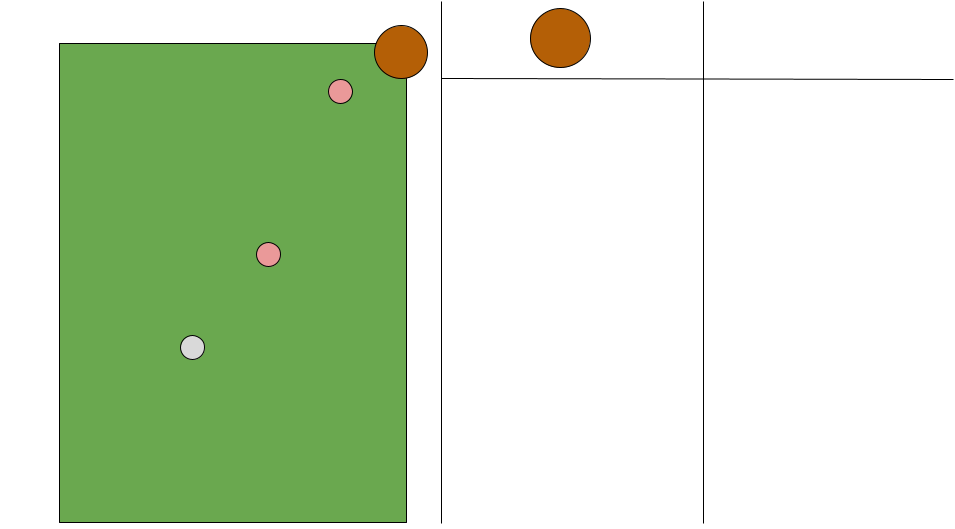
\includegraphics[width=0.5\linewidth]{../common/03_billiard_ai/resources/11_backwardsearch_1.png}
    \end{center}
    \caption{Kandidatensuche 1: Links ist der Spielstand auf dem Billardtisch abgebildet. Auf der rechten Seite des Tisches ist der Suchbaum dargestellt.
    Im ersten Schritt wurden ausgehend vom Zielloch noch keine Kugeln expandiert.
    Es stehen die beiden roten Kugeln zur Auswahl.}
    \label{fig:backwardsearch_1}
\end{figure}

In einem zweiten Schritt wird die einzulochende Kugel definiert. Es kommen lediglich die beiden roten Kugeln in Frage.
Nachfolgend wird der Pfad weiter betrachtet, bei dem die beim Loch näherstehende rote Kugel, gewählt wurde.
Abbildung \ref{fig:backwardsearch_2} zeigt, dass der Suchbaum um einen Knoten erweitert wurde.
\begin{figure}[h!]
    \begin{center}
        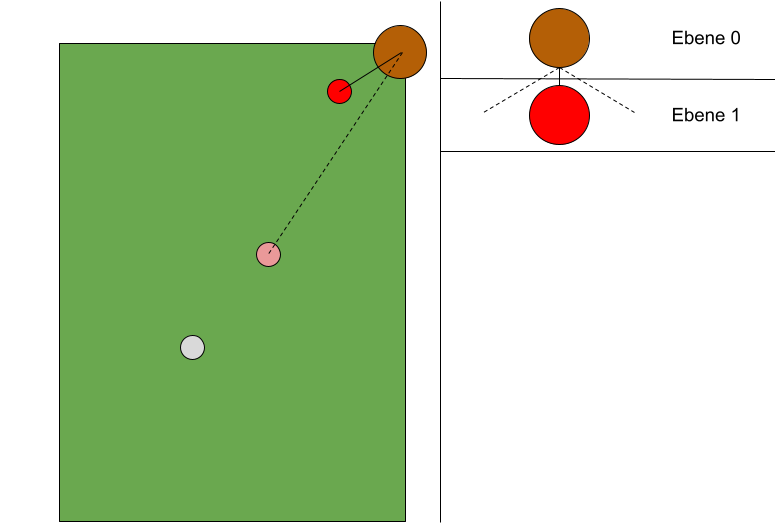
\includegraphics[width=0.5\linewidth]{../common/03_billiard_ai/resources/12_backwardsearch_2.png}
    \end{center}
    \caption{Kandidatensuche 2: Im ersten Expansionsschritt wurde die dunkelrot eingefärbte Kugel als einzulochende Kugel gewählt.
    Im Suchbaum ist diese dadurch als Knoten eingefügt worden. }
    \label{fig:backwardsearch_2}
\end{figure}

In Abbildung \ref{fig:backwardsearch_3} erfolgt der letzte Schritt. Hier sind verschiedene Optionen möglich, bspw.
könnte die weisse Kugel direkt oder über die Bande an die zuvor gewählte rote Kugel gespielt werden. Es könnte aber auch
die andere rote Kugel an die zuvor gewählte rote Kugel gespielt werden. Hier wird der Fall betrachtet, dass die weisse Kugel
indirekt über eine Bande an die zuvor gewählte rote Kugel gespielt wird.
\begin{figure}[h!]
    \begin{center}
        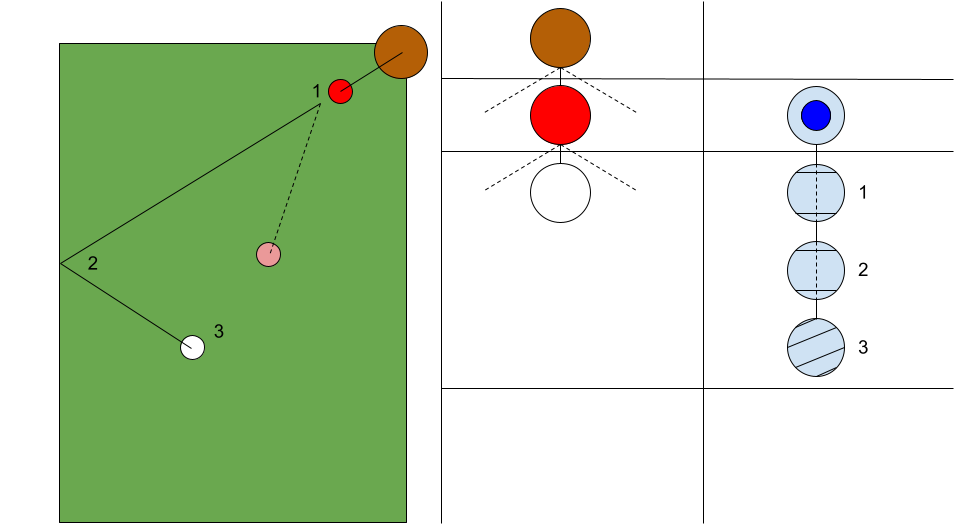
\includegraphics[width=0.5\linewidth]{../common/03_billiard_ai/resources/13_backwardsearch_3.png}
    \end{center}
    \caption{Kandidatensuche 3: Im letzten Expansionsschritt wurde die weisse Kugel gewählt und wird über die Bande an die rote Kugel gespielt.
    Der Suchbaum hat demnach einen neuen Knoten für die weisse Kugel, wodurch ein Pfad für einen vollständiger Stoss entstanden ist.}
    \label{fig:backwardsearch_3}
\end{figure}

Algorithmus \ref{alg:backward_search} verdeutlicht den Ablauf der \glqq Expand-Funktion\grqq. Zuerst wird eine
leere Liste namens \glqq nodes\grqq{} angelegt. Diese wird danach mit Nodes gefüllt, welche entweder durch einen Stoss
über eine weitere Kugel oder indirekt über die Bande zustande kommen. Die Nodes bilden das Ergebnis der Funktion.

\begin{algorithm}[H]
    \DontPrintSemicolon
    \SetKwFunction{expand}{expand}
    \SetKwProg{Fn}{Function}{}{}
    \Fn{\expand{node: Node, constantObjects: list} $\longrightarrow$ list[Node]}{
        nodes $\longleftarrow$ list()\\
        nodes $\longleftarrow$ append(expandBalls(node, constantObjects), nodes)\\
        nodes $\longleftarrow$ append(expandBank(node, constantObjects), nodes)\\
        \KwRet nodes
    }
    \caption{Algorithmus zur Durchführung eines Expansionsschritts bei der Kandidatensuche}
    \label{alg:backward_search}
\end{algorithm}

\subsubsection{Expansion einer Kugel}
In der anzuwendenden Graphensuche müssen die nächsten Knoten expandiert werden.
Eine Expansion kann über eine Kugel- oder über eine Bandenkollision stattfinden.

\paragraph{Expansion über eine Kugelkollision}\mbox{}\\

Bei einer Expansion einer Kugel wird der nächste Zielpunkt berechnet.
Das Prinzip wird in Abbildung \ref{fig:kugelexpansion} veranschaulicht.
Der Zielpunkt $T$, wohin die Kugel gespielt werden soll, ist bekannt.
Weiterhin ist die aktuelle Position $S$ der Kugel bekannt. Dazwischen kann der Vektor $\vec{d}$ gebildet werden.
\begin{align}
    \vec{d} = S - T
\end{align}
Damit die Kugel in Richtung des Zielpunkts $T$ rollt, muss diese von einer anderen Kugel am Punkt $Z$ angestossen werden.
Daher gilt es $Z$ zu bestimmen.
Der neue Zielpunkt $Z$ wird mithilfe des Vektors $d$ und dem bekannten Kugelradius $r$ berechnet.
\begin{align}
    Z = S + 2 \cdot r \cdot \hat{d}
\end{align}

\begin{figure}[h!]
    \begin{center}
        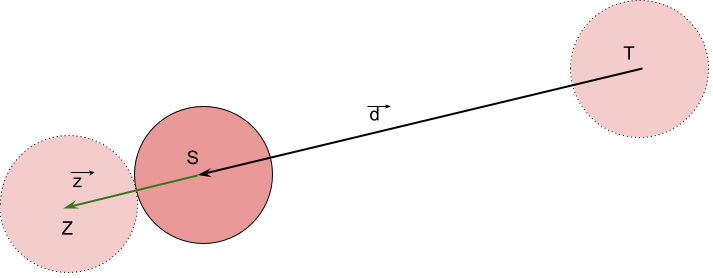
\includegraphics[width=0.5\linewidth]{../common/03_billiard_ai/resources/35_suchkandidat_kugel_expand.png}
    \end{center}
    \caption{Kugelexpansion}
    \label{fig:kugelexpansion}
\end{figure}

\paragraph{Expansion über eine Bandenkollision}\label{kandidatensuche:bandenkollisionstheorie}\mbox{}\\

Eine Kugel kann ebenso über eine oder mehrere Banden expandiert werden. Dazu muss bekannt sein, wie der Verlauf einer
Kugel nach einer Bandenkollision aussieht. Um diese Frage beantworten zu können, wurden zwei Arbeiten betrachtet.
Nach diesen Quellen gilt für den Stoss einer Kugel über die Bande, dass im Falle eines nicht vorhandenen Spins
der Ausfallswinkel dem Einfallswinkel entspricht. Dieses Verhalten wurde von den Autoren des Papers \glqq A theoretical analysis of billiard ball dynamics under cushion impacts\grqq{}
untersucht \cite{10.1243/09544062JMES1964}.
Der Abschnitt \glqq b\grqq{} der Abbildung \ref{fig:rail_rebound_angle_no_spin} zeigt die
funktionale fast lineare Abhängigkeit des Ausfallswinkels vom Einfallswinkel.
Diese Werte wurden anhand verschiedener Geschwindigkeiten in praktischen Experimenten ermittelt \cite{10.1243/09544062JMES1964}.

\begin{figure}[h!]
    \begin{center}
        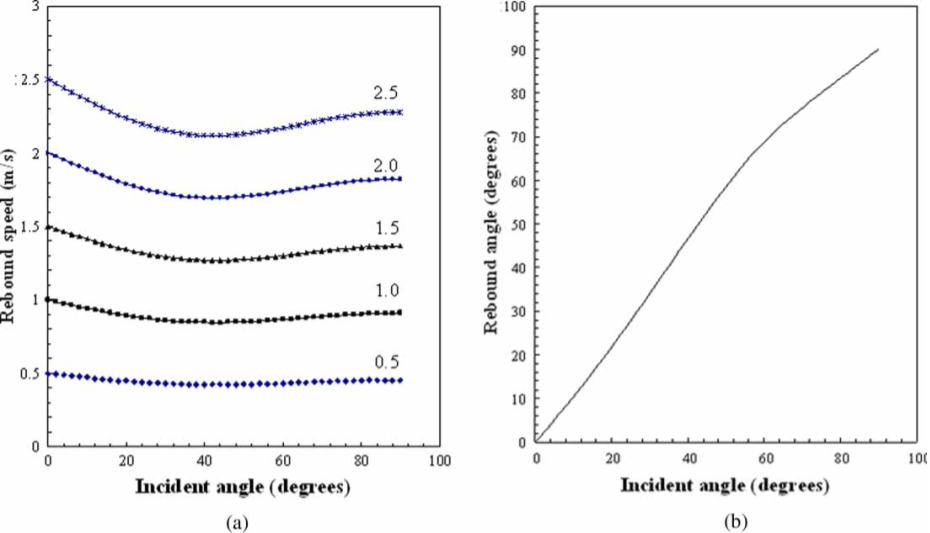
\includegraphics[width=0.5\linewidth]{../common/03_billiard_ai/resources/55_rail_rebound_angle_no_spin.png}
    \end{center}
    \caption{Geschwindigkeits- und Ausfallswinkelabhängigkeiten zum Einfallswinkel einer Kugel ohne Spin an einer Bande.
    Entnommen aus der Arbeit \cite{10.1243/09544062JMES1964} des Kapitels \glqq Results and Discussion\grqq. }
    \label{fig:rail_rebound_angle_no_spin}
\end{figure}

Eine weitere Bestätigung und eine ebenso ausführliche Behandlung des Themas findet sich im Buch \glqq The illustrated principles
of pool and billiards\grqq. Auch dieser Arbeit liegen praktische
\href{https://billiards.colostate.edu/high-speed-video/}{Experimente} zugrunde, die die Theorie bestätigen.
Grundsätzlich gilt das Prinzip 6.1 \glqq Bank shot geometry\grqq, welches besagt, dass
der Ausfallswinkel dem Einfallswinkel entspricht, dies ist
jedoch bei schwachen und starken wie auch bei Stössen der Bande sehr nahe liegenden Kugeln nicht korrekt \cite{book:the_ilustrated_principles_of_pool_and_billiards}.
So besagt das Prinzip 6.6 \glqq Rail throwback at high speed\grqq, dass der Ausfallswinkel kleiner wird, je stärker der Stoss ausgeführt wird.
Dieser Effekt tritt vor allem bei Einfallswinkeln zwischen $20^{\circ}$ und $50^{\circ}$ auf und ist auf
die seitliche Kompression der Bande zurückzuführen. Diese wird unterschiedlich stark eingedrückt und gibt durch die
darauffolgende Entspannung eine stärkere Kraft in die einfallende Richtung der Kugel zurück \cite{book:the_ilustrated_principles_of_pool_and_billiards}.
Dieser Umstand wird in der Abbildung \ref{fig:rebound_angle_no_spin_fast_shot} gezeigt.

\begin{figure}[h!]
    \begin{center}
        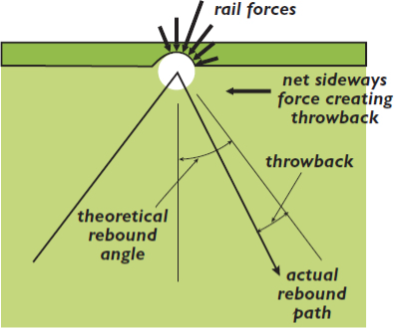
\includegraphics[width=0.3\linewidth]{../common/03_billiard_ai/resources/56_rebound_angle_no_spin_fast_shot.png}
    \end{center}
    \caption{Unterschiedliche Belastung der Bande bei starkem Stoss einer Kugel.
    Entnommen aus dem Buch \cite{book:the_ilustrated_principles_of_pool_and_billiards} des Kapitels \glqq 6 Bank and kick shots\grqq.}
    \label{fig:rebound_angle_no_spin_fast_shot}
\end{figure}

Trifft die Kugel langsam auf die Bande auf, so gilt Prinzip 6.7 \glqq Curved rebound path due to slow-speed roll\grqq.
Dieses verweist auf den Umstand, dass eine Kugel, die langsam auf die Bande trifft, aufgrund des resultierenden
Topspins kurvenförmig wegrollt. Der Effekt ist bei einem Einfallswinkel von $45^{\circ}$ am stärksten \cite{book:the_ilustrated_principles_of_pool_and_billiards}.
Die Abbildung \ref{fig:rebound_angle_no_spin_slow_shot} verdeutlicht das Prinzip.

\begin{figure}[h!]
    \begin{center}
        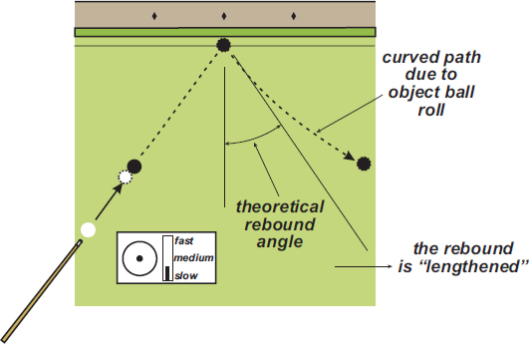
\includegraphics[width=0.4\linewidth]{../common/03_billiard_ai/resources/57_rebound_angle_no_spin_slow_shot.png}
    \end{center}
    \caption{Einfluss des Topspins auf den Ausfallswinkel bei schwachem Stoss einer Kugel an eine Bande.
    Entnommen aus dem Buch \cite{book:the_ilustrated_principles_of_pool_and_billiards} des Kapitels \glqq 6 Bank and kick shots\grqq.}
    \label{fig:rebound_angle_no_spin_slow_shot}
\end{figure}

Trifft eine Kugel langsam auf die Bande auf und ist sehr nahe, so dass sie zum Zeitpunkt der Kollision noch nicht zu rollen begonnen hat,
gilt Prinzip 6.8 \glqq Smaller rebound angle when close to the rail\grqq.
Dieses besagt, dass der Ausfallswinkel demnach kleiner wird \cite{book:the_ilustrated_principles_of_pool_and_billiards}.
Der resultierende Unterschied aufgrund der Distanzen wird in Abbildung \ref{fig:rebound_angle_no_spin_slow_shot_distance} veranschaulicht.

\begin{figure}[h!]
    \begin{center}
        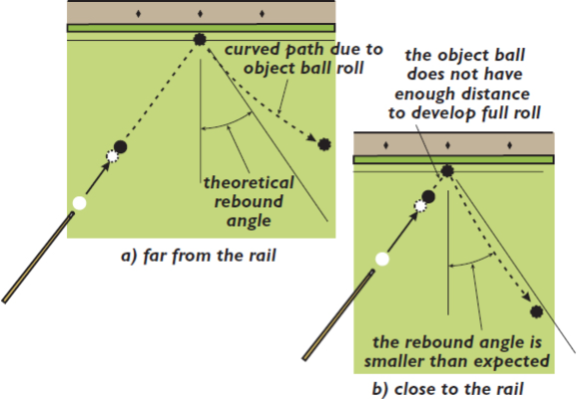
\includegraphics[width=0.4\linewidth]{../common/03_billiard_ai/resources/58_rebound_angle_no_spin_slow_shot_distance.png}
    \end{center}
    \caption{Einfluss der Distanz auf den Ausfallswinkel bei schwachem Stoss einer Kugel an eine Bande.
    Entnommen aus dem Buch \cite{book:the_ilustrated_principles_of_pool_and_billiards} des Kapitels \glqq 6 Bank and kick shots\grqq.}
    \label{fig:rebound_angle_no_spin_slow_shot_distance}
\end{figure}

\newpage
Aufgrund dieser Erkenntnisse und der gegebenen Abhängigkeit wird der Ausfallswinkel dem Einfallswinkel gleichgesetzt.
Technisch geschieht dies über einen geometrischen Ansatz durch eine Spiegelung \cite{math.stackexchange:1}
des Zielpunkts an der entsprechenden Bande, über welche gespielt werden soll.
In Abbildung \ref{fig:Tiefe über Bande erreichen mittels Reflektion} wird ein Suchschritt über eine Bande visualisiert.
Es wird ein Punkt $A$ an einer Bande gesucht, zu welchem die Kugel $B$ gespielt werden muss, um die Kugel $C$ zu treffen.
Dieser Bandenkollisionspunkt $A$ wird mithilfe eines Spiegelpunkts $\bar{C}$ des Punktes $C$ an der Bande berechnet.

\begin{figure}[h!]
    \begin{center}
        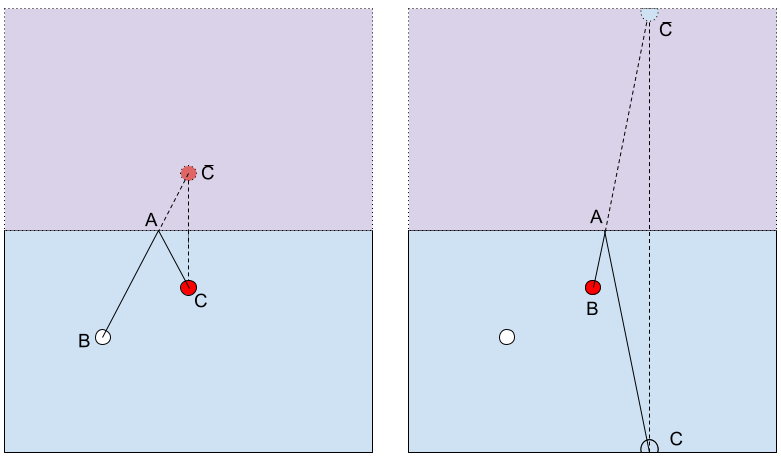
\includegraphics[width=0.5\linewidth]{../common/03_billiard_ai/resources/47_rail_reflection_1.png}
    \end{center}
    \caption{Zwei Fälle für ein Bandenspiel:
    Im ersten Fall wird für die weisse Kugel ein Kollisionspunkt an der oberen Bande bestimmt, um die rote Kugel zu treffen.
    Im zweiten Fall wird für die rote Kugel ein Kollisionspunkt an der oberen Bande bestimmt, um ins Ziel zu treffen.
    }
    \label{fig:Tiefe über Bande erreichen mittels Reflektion}
\end{figure}

Gegeben sind die folgenden Angaben (Parameter werden grossgeschrieben, Variablen dagegen klein):
\begin{align}
    B = \begin{pmatrix}B_X\\B_Y\end{pmatrix},
    C = \begin{pmatrix}C_X\\C_Y\end{pmatrix},
    \bar{C} = \begin{pmatrix}\bar{C_X}\\\bar{C_Y}\end{pmatrix},
\end{align}
Der Schnittpunkt kann über zwei Geraden berechnet werden, die über die Parameterform gegeben sind.
Eine dieser Geraden liefert der gespiegelte Punkt $\bar{C}$ mit $B$.
\begin{align}
    \vec{l} = \vec{\bar{C}} - \vec{B}\\
    L_1 = \vec{B} + \lambda_1 \cdot \vec{l}
\end{align}
Die andere Gerade ist über die Bande (Rail) gegeben, wobei $R_1$ der Startpunkt und $R_2$ der Endpunkt der Bande ist:
\begin{align}
    R_1 = \begin{pmatrix}R_{1X}\\R_{1Y}\end{pmatrix}, R_2 = \begin{pmatrix}R_{2X}\\R_{2Y}\end{pmatrix}\\
    \vec{r} = \vec{R_2} - \vec{R_1}\\
    L_2 = \vec{R_1} + \lambda_2 \cdot \vec{r}
\end{align}
Der Kollisionspunkt $A$ lässt sich über $\lambda_1$ der Gleichung \ref{eq:bandenkollisionspunkt} mithilfe der Linie $L_1$
bestimmen (Herleitung, siehe Anhang \ref{anhang:herleitung:bandenreflektion}).

\begin{align}
    \lambda_1 = \frac{r_x \cdot B_y - r_y \cdot B_x + R_{1,x} \cdot r_y - R_{1,y} \cdot r_x}{l_x \cdot r_y - \cdot l_y \cdot r_x}\label{eq:bandenkollisionspunkt}
\end{align}

Es gilt zu beachten, dass es sich bei der Billardkugel nicht um einen unendlich kleinen Punkt handelt und
daher deren Radius berücksichtigt werden muss.
Das Problem wird in Abbildung ~\ref{fig:bandenreflektion_kugelradius} dargestellt.
\begin{figure}[h]
    \begin{center}
        \includegraphics[width=0.5\linewidth]{../common/03_billiard_ai/resources/48_bandenreflektion_kugelradius.png}
    \end{center}
    \caption{Berücksichtigung des Kugelradius bei Bandenreflektion: Die Bande wird um den Kugelradius in Richtung Tischmitte verschoben.}
    \label{fig:bandenreflektion_kugelradius}
\end{figure}

Einerseits wird als Zielposition $C$ nicht die Kugelposition selbst, sondern ein um den Radius verschobener Punkt in
Gegenrichtung zur gewünschten Laufrichtung $\vec{r}$ der Kugel $C$ definiert. Andererseits wird die Bande, an welcher
gespiegelt wird, um den Radius der Kugel in Richtung des Zentrums verschoben. Die verschobene virtuelle Bande ist grün eingezeichnet.

Durch Studium mehrerer Beispiele wird ein allgemeiner Algorithmus hergeleitet. Hierbei wird das zuvor genannte Problem
mit dem Kugelradius vernachlässigt, da dieses durch die beschriebenen Positionskorrekturen behandelt werden kann.
Der Algorithmus kann unabhängig von dieser Korrektur beschrieben werden.

In einem ersten Schritt werden die Banden definiert, über welche der Zielpunkt gespiegelt werden soll. Dies sind in
diesem Beispiel die linke und die obere Bande, dementsprechend werden die grün markierten Spiegel zuerst links und
dann oben angewendet. Es resultieren die Punkte $\bar{C_0}$ und $\bar{C_1}$. Die Abbildung \ref{fig:zweifaches_bandenspiel_a} zeigt die
Situation mitsamt der gespiegelten Punkte.
\begin{figure}[h]
    \begin{center}
        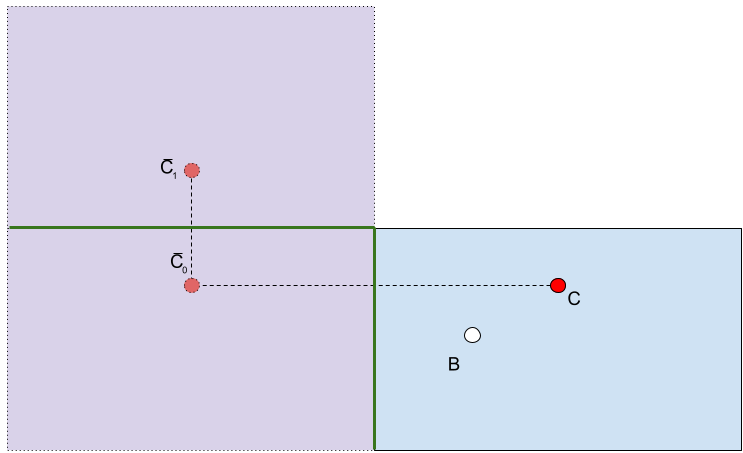
\includegraphics[width=0.5\linewidth]{../common/03_billiard_ai/resources/50_rail_reflection_2_a.png}
    \end{center}
    \caption{Zweifaches Bandenspiel - A: Der Zielpunkt C wurde zuerst an der linken, dann an der oberen Bande gespiegelt.}
    \label{fig:zweifaches_bandenspiel_a}
\end{figure}

Die Abbildung \ref{fig:zweifaches_bandenspiel_b} zeigt das Vorgehen, nachdem die Spiegelungen durchgeführt wurden.
Es wird der letzte Spiegelpunkt $\bar{C_n}$, in diesem Fall $\bar{C_1}$,
beibehalten, die Vorherigen werden verworfen. Vom Startpunkt $B$ aus wird eine Verbindung zum Spiegelpunkt $\bar{C_1}$
gezogen und alle Bandensegmente auf Schnittpunkte geprüft, was schliesslich im Punkt $A_0$ resultiert. Dies ist
der erste Kollisionspunkt mit der Bande und kann der Resultatsmenge hinzugefügt werden. Anschliessend wird der Spiegelpunkt
$\bar{C_1}$ an der Bande gespiegelt, an welcher der Kollisionspunkt liegt, in dem Fall an der Linken. Diese Spiegelung
resultiert im Spiegelpunkt $\bar{C_0}$.
\begin{figure}[h]
    \begin{center}
        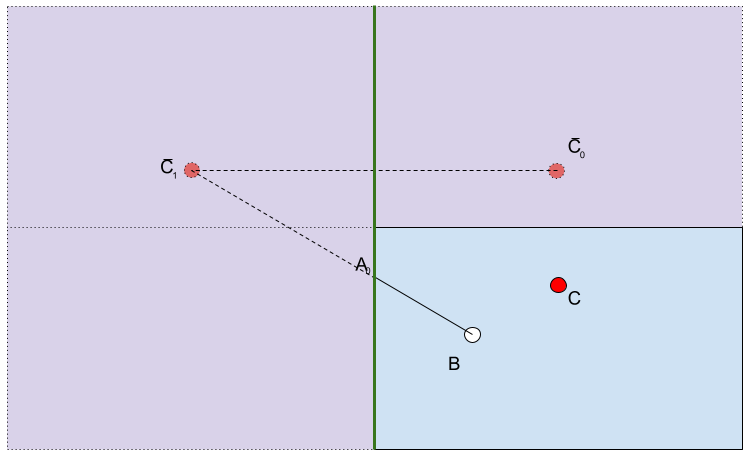
\includegraphics[width=0.5\linewidth]{../common/03_billiard_ai/resources/51_rail_reflection_2_b.png}
    \end{center}
    \caption{Zweifaches Bandenspiel - B: Der Schnittpunkt $A-0$ an der linken Bande ist der erste Bandenkollisionspunkt.
    Um den zweiten Bandenkollisionspunkt zu bestimmen, wird die Spiegelung an der linken Bande rückgängig gemacht.}
    \label{fig:zweifaches_bandenspiel_b}
\end{figure}

In der Abbildung \ref{fig:zweifaches_bandenspiel_c} ist der darauffolgende Schritt ersichtlich.
Es gibt zum Vorhergehenden keine wesentlichen Unterschiede.
Es wird wiederum nur der letzte Spiegelpunkt $\bar{C_0}$ beibehalten, zu welchem vom
neuen Startpunkt $A_0$ eine Verbindung gezogen wird.
Diese Halbgerade wird wiederum auf Schnittpunkte mit allen Bandensegmenten geprüft, was im Kollisionspunkt $A_1$ resultiert.
Dieser Kollisionspunkt wird der Resultatsmenge hinzugefügt und der Punkt $\bar{C_0}$
wird an der Bande mit dem Kollisionspunkt gespiegelt, in dem Fall der Oberen.
Diese Spiegelung überführt den Punkt $\bar{C_0}$ auf den ursprünglichen Punkt $C$, was das Ende des Algorithmus
bedeutet.
\begin{figure}[h]
    \begin{center}
        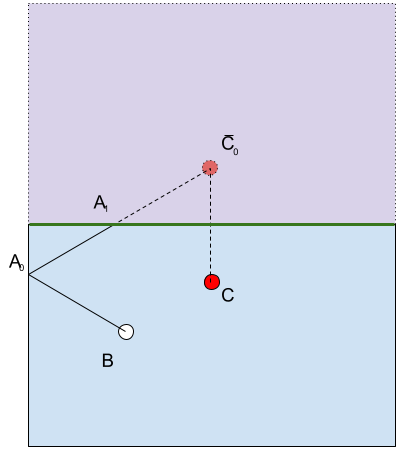
\includegraphics[width=0.5\linewidth]{../common/03_billiard_ai/resources/52_rail_reflection_2_c.png}
    \end{center}
    \caption{Zweifaches Bandenspiel - C: Der Schnittpunkt $A-1$ an der oberen Bande ist der zweite Bandenkollisionspunkt.
    Wenn die Spiegelung an der oberen Bande rückgängig gemacht wird, fällt der Zielpunkt wieder auf den ursprünglichen Punkt C zurück.}
    \label{fig:zweifaches_bandenspiel_c}
\end{figure}

Die Abbildung \ref{fig:zweifaches_bandenspiel_d} zeigt das endgültige Resultat, wenn der letzte Kollisionspunkt $A_1$
mit dem Zielpunkt $C$ verbunden wird.

\begin{figure}[h!]
    \begin{center}
        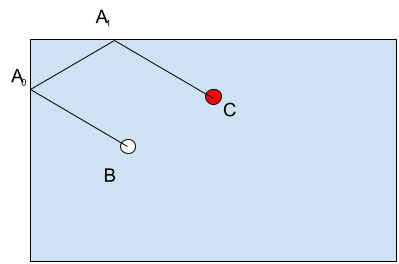
\includegraphics[width=0.5\linewidth]{../common/03_billiard_ai/resources/53_rail_reflection_2_d.png}
    \end{center}
    \caption{Zweifaches Bandenspiel - D: Die weisse Kugel wird von B über $A_0$ und $A_1$ an die rote Kugel an Position C gespielt.}
    \label{fig:zweifaches_bandenspiel_d}
\end{figure}

Dasselbe Prinzip kann auch auf ein Spiel über drei Banden angewendet werden, siehe Abbildung \ref{fig:Dreifache Reflektion an Banden}.
Es wird zuerst an der linken, dann an der oberen und anschliessend an der rechten Bande gespiegelt.
Es wird in einem Schritt wiederum der letzte Spiegelpunkt und dessen Startposition betrachtet, mit welchen der Kollisionspunkt
an einer Bande gefunden werden kann. Danach kann der Spiegelpunkt an dieser Bande gespiegelt werden und der nächste
Schritt kann starten. Dies wird so oft wiederholt, wie es Banden zum Spiegeln hat.
\begin{figure}[h]
    \begin{center}
        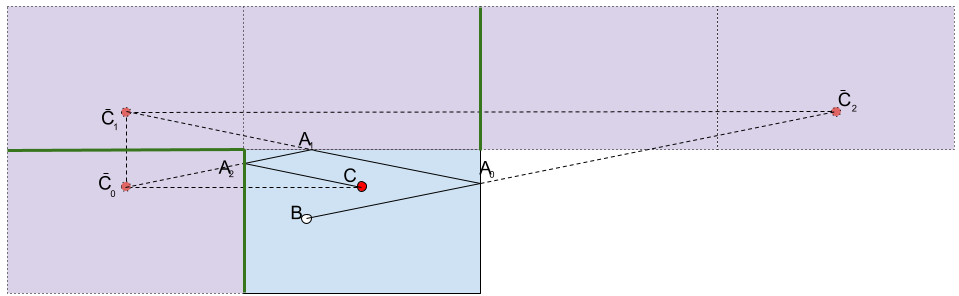
\includegraphics[width=1\linewidth]{../common/03_billiard_ai/resources/54_rail_reflection_3.png}
    \end{center}
    \caption{Dreifache Reflektion an Banden. Es wird zuerst an der linken, dann an der oberen und zuletzt an der rechten Bande gespiegelt.}
    \label{fig:Dreifache Reflektion an Banden}
\end{figure}

Eine Spiegelung kann durch die Anwendung der bandenspezifischen Transformationsmatrix $M$ erzielt werden, wobei $\vec{s}$
für den Spiegelvektor steht (Herleitung, siehe Anhang \ref{anhang:herleitung:bandenreflektion:zielpunkt}).
Hierbei steht der Punkt $C$ für den Zielpunkt, den es zu treffen gilt.
\begin{align}
    M = \begin{pmatrix}s_x & 0 & R^1_x - s_x \cdot R^1_x \\ 0 & s_y & R^1_y - s_y \cdot R^1_y \\ 0 & 0 & 1\end{pmatrix}\\
    \bar{C} = M \cdot C
\end{align}

Weiterhin stellt sich die Frage, an welcher Bande überhaupt gespiegelt werden darf.
Dazu wurden Definitionsbereiche für jede Bande erstellt, wie in Abbildung \ref{fig:Definitionsbereich_Bandenspiegelung} ersichtlich ist.
Punkte auf der roten Seite liegen ausserhalb des Definitionsbereichs, Punkte im grünen Bereich sind spiegelbar.
Des Weiteren ist die Bandennormale vorhanden, welche zum Ursprung des Koordinatensystems in der Tischmitte zeigt.

\begin{figure}[h!]
    \begin{center}
        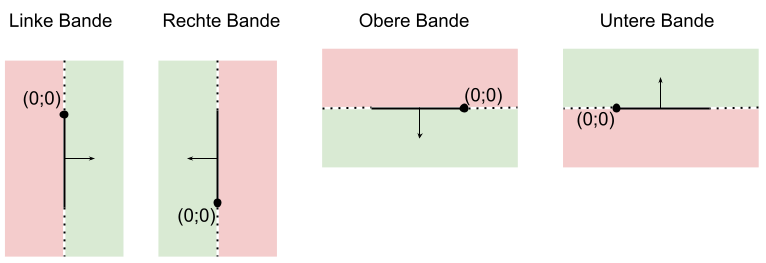
\includegraphics[width=1\linewidth]{../common/03_billiard_ai/resources/49_definitionsbereich_spiegelung_bande.png}
    \end{center}
    \caption{Definitionsbereich einer Bandenspiegelung. Wenn sich ein Zielpunkt im roten Bereich befindet, kann dieser nicht über die Bande angespielt werden.}
    \label{fig:Definitionsbereich_Bandenspiegelung}
\end{figure}

Um für einen Punkt $C$ herauszufinden, ob dieser spiegelbar ist, muss nur geprüft werden, ob er im Definitionsbereich liegt.
Dazu wird der Ursprung des Koordinatensystems zum Start der Bande verschoben und es wird die elementweise Multiplikation
des verschobenen Punktes $C'$ mit der Bandennormale durchgeführt.
Die Elemente des Vektors werden geprüft, ob sie grösser oder gleich dem Nullvektor sind.
Dies resultiert in einem Vektor, welcher eine $0$ speichert, wenn das Element kleiner und $1$, wenn es grösser ist.
Abschliessend wird die quadrierte Länge des resultierenden Vektors gebildet, diese Länge muss $2$ entsprechen, in dem
Fall liegt der Punkt im Definitionsbereich.
\begin{align}
    C^{'} = C \cdot T^0\\
    \bar{C} = C^{'} \cdot \hat{n}\\
    \vec{r} = \bar{C} \geq \vec{0}\\
    l = \vec{r} \cdot \vec{r}\\
    p = l == 2
\end{align}

Wird ein Punkt geprüft, der auf derselben Höhe wie eine Bande liegt, muss zusätzlich die jeweilige Komponente des Punktes
$\bar{C}$ grösser als $0$ sein, bei der die Komponente des Normalenvektors ungleich $0$ ist.

\clearpage
Algorithmus \ref{alg:stoss_ueber_bande_1} und \ref{alg:stoss_ueber_bande_2} zeigt, wie ein Stoss über die Bande gefunden werden kann.
Dazu werden in einem ersten Schritt alle möglichen Kombinationen der Banden gebildet, was auch den letzten Spiegelpunkt
$\bar{C_n}$ generiert. Danach können die Zielpositionen bestimmt werden, wobei auch geprüft wird, ob der Weg zwischen
den Positionen passierbar ist. Sollte dies nicht der Fall sein, wird dieser Lösungskandidat verworfen.

\begin{algorithm}[H]
    \DontPrintSemicolon
    \SetKwFunction{expandByRail}{expandByRail}
    \SetKwFunction{combos}{combos}
    \SetKwFunction{canReflect}{canReflect}
    \SetKwFunction{reflect}{reflect}
    \SetKwProg{Fn}{Function}{}{}
    \Fn{\expandByRail{B: vec2, C: vec2, reflections: int, rails: Rail[]} $\longrightarrow$ Node[]}{
        nodes $\longleftarrow$ Node[]\\
        combinations $\longleftarrow$ combos(reflections, C, rails)\\
        \For{combination in combinations}{
            targets $\longleftarrow$ target(B, C, combination.second,rails, combination.first)\\

            \If{! empty(targets)}{
                nodes $\longleftarrow$ append(physicalEvents(B, C, targets), nodes)
            }
        }
        \KwRet nodes
    }
    \;
    \Fn{\combos{reflections: int, target: vec2, rails: Rail[]} $\longrightarrow$ (Rail[], vec2)[]}{
        combinations: (Rail[], vec2, bool)[] $\longleftarrow$ []\\
        \For{rail in rails}{
            combinations $\longleftarrow$ append(([rail], reflect(target, rail), canReflect(target, rail)), combinations)
        }
        \For{index $\longleftarrow$ 1 < reflections}{
            \For{railIndex $\longleftarrow$ 0 < length(rails)}{
                rail $\longleftarrow$ rails[railIndex]\\
                \If{combinations[railIndex].third and canReflect(combinations[railIndex].second, rail)}{
                    combinations[railIndex].first $\longleftarrow$ append(rail, combinations[railIndex].first)\\
                    combinations[railIndex].second $\longleftarrow$ reflect(combinations[railIndex].second, rail)
                }
                \Else{
                    combinations[railIndex].third $\longleftarrow$ false
                }
            }
        }

        results: (Rail[], vec2)[] $\longleftarrow$ []\\
        \For{railIndex $\longleftarrow$ 0 < length(rails)}{
            \If{combinations[railIndex].third}{
                results $\longleftarrow$ append((combinations[railIndex].first, combinations[railIndex].second), results)
            }
        }

        \KwRet results
    }
    \;
    \Fn{\canReflect{C: vec2, rail: Rail} $\longrightarrow$ bool}{
        moved $\longleftarrow$ C $-$ rail.start\\
        reflected $\longleftarrow$ moved $\cdot$ rail.normal\\
        possible $\longleftarrow$ reflected $\geq \vec{0}$\\
        \KwRet possible $\cdot$ possible $= 2$
    }
    \;
    \Fn{\reflect{C: vec2, rail: Rail} $\longrightarrow$ vec2}{
        reflected: vec3 $\longleftarrow$ vec3(C, 1.0)\\
        \KwRet vec2(rail.M $\cdot$ reflected)
    }
    \caption{Algorithmus zur Berechnung eines Stosses über die Bande - Teil 1}
    \label{alg:stoss_ueber_bande_1}
\end{algorithm}
\newpage
\begin{algorithm}[H]
    \DontPrintSemicolon
    \SetKwFunction{target}{target}
    \SetKwProg{Fn}{Function}{}{}
    \Fn{\target{B: vec2, C: vec2, reflected: vec2, rails: Rail[], combo: Rail[]} $\longrightarrow$ vec2[]}{
        targets $\longleftarrow$ vec2[]\\
        start $\longleftarrow$ B\\
        \While{! empty(combo)}{
            comboRail $\longleftarrow$ pop(combo)\\
            target $\longleftarrow$ $(\infty, \infty)$\\
            \For{rail in rails}{
                railIntersection $\longleftarrow$ halfLineLineSegmentIntersection(start, (reflected - start), rail.start, rail.end)\\
                \If{railIntersection and start <> railIntersection}{
                    target $\longleftarrow$ railIntersection\\
                    reflected $\longleftarrow$ reflect(reflected, rail)\\
                    break
                }
            }
            \If{! shotPossible(start, target)}{
                \KwRet {}
            }
            targets $\longleftarrow$ append(target, targets)\\
            start $\longleftarrow$ target\\
        }

        If{! shotPossible(start, C)}{
            \KwRet {}
        }
        \KwRet targets
    }
    \caption{Algorithmus zur Berechnung eines Stosses über die Bande - Teil 2}
    \label{alg:stoss_ueber_bande_2}
\end{algorithm}

\paragraph{Prüfung der Ausführbarkeit eines Stosses}\mbox{}\\

Für die Expansion einer Kugel, sei es über eine weitere Kugel oder über eine Bande,
muss geprüft werden, dass keine weitere Kugel im Weg ist. Dies wird über die Berechnung
des Distanzvektors zwischen dem Vektor $\vec{d}$ und der zu prüfenden Kugel erzielt. Dasselbe Prinzip wird
in Kapitel \ref{kap:kugelkollision:performanceverbesserung} beim Fall einer dynamisch-statischen Kugelkollision erläutert.

%Bei der Prüfung auf eine mögliche Bandenkollision zwischen der aktuellen Position und dem Zielpunkt muss der Durchmesser
%der Kugel mitberücksichtigt werden. Eine mögliche Situation wird in Abbildung \ref{fig:kugelexpansion_bandenkollision} dargestellt.
%Dazu die Bande $R$ in Normalenrichtung verschoben, wobei die Normale in Richtung des Koordinatenursprungs zeigt. Es resultiert
%die virtuelle Bande $R_V$. Da die Bande durch zwei Punkte (Start und Ende) definiert ist, kann eine Gerade beschrieben werden.
%Dies gilt ebenso für die Kugel $K_1$. Deren Geradengleichung lautet:
%\begin{align}
%    K_1(\lambda) = S - \lambda \cdot \hat{d}
%\end{align}
%Ein Schnittpunkttest zwischen diesen Geraden sollte kein Ergebnis liefern, ansonsten wird vor dem Erreichen des Zielpunkts
%$T$ eine Kollision mit der Bande stattfinden, wie es in diesem Szenario der Fall ist.

%\begin{figure}[h!]
%    \begin{center}
%        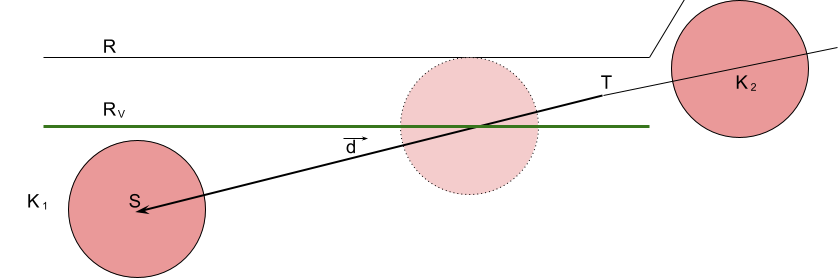
\includegraphics[width=0.5\linewidth]{../common/03_billiard_ai/resources/36_suchkandidat_kugel_expand_banden_kollision.png}
%    \end{center}
%    \caption{Kugelexpansion - Bandenkollision}
%    \label{fig:kugelexpansion_bandenkollision}
%\end{figure}

Sobald die weisse Kugel expandiert wird, muss sichergestellt werden, dass diese auch an der entsprechenden Position
mit dem Queue getroffen werden kann.
Dies wird, wie in Abbildung \ref{fig:kugelexpansion_platz_fuer_queue} veranschaulicht,
durch einen Vektor $\vec{s}$ mit einer bestimmten Länge $s$ entgegen der Rollrichtung der Kugel sowie einem Mindestabstand
$e$ zu diesem Vektor sichergestellt. Die Länge von $e$ wird auf $10 [mm]$ gewählt. Von jeder Kugel aus
werden die Abstände gemessen, liegt die Kugel zwischen $W$ und $W + \vec{s}$, so wird der Abstand senkrecht zum Vektor $\vec{s}$
berechnet, zu sehen bei der Kugel $K_1$. Liegt die Kugel wie $K_2$ vorne oder hinten, wird der Abstand zum Punkt $W$ oder $W + \vec{s}$
berechnet. Für die so erhaltenen Distanzen $d_i$ muss gelten, wobei $r$ für den Kugelradius steht:
\begin{align}
    d_i >= e + r
\end{align}

Liegt die Kugel in Richtung der Rollrichtung, wurde die Bedingung bereits geprüft, ansonsten dürfte die weisse Kugel nicht
expandiert worden sein. Daher muss dieser Fall nicht speziell behandelt werden.

\begin{figure}[h!]
    \begin{center}
        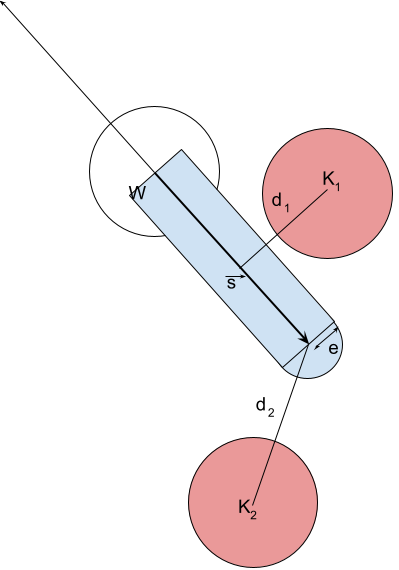
\includegraphics[width=0.3\linewidth]{../common/03_billiard_ai/resources/37_platz_fuer_queue.png}
    \end{center}
    \caption{Kugelexpansion - Platz für Queue. Der blau hinterlegte Bereich hinter der weissen Kugel darf nicht von anderen Kugeln belegt sein,
        damit diese mithilfe des Queues wie gewünscht angestossen werden kann.}
    \label{fig:kugelexpansion_platz_fuer_queue}
\end{figure}

\newpage
\subsubsection{Bewertungsfunktion}
Um die Suche zu vereinfachen und in eine spezifische Richtung zu lenken, wo die besten Resultate zu erwarten sind, ist
es unerlässlich eine Bewertung des Stosses durchzuführen.
Die Bewertungsfunktion wurde so definiert, dass sie sich auf den aktuell expandierten Knoten beschränkt.
Die Kosten für eine Expansion werden über die Pfade aufsummiert.
Anhand der Summen kann jeweils der kostengünstigste Pfad evaluiert und verfolgt werden.
Abbildung \ref{fig:suchbaum_bewertung} zeigt das Prinzip.
Dieses Vorgehen entspricht demjenigen des Dijkstra-Algorithmus \cite{wiki.dijkstra:1}.
\begin{figure}[h!]
    \begin{center}
        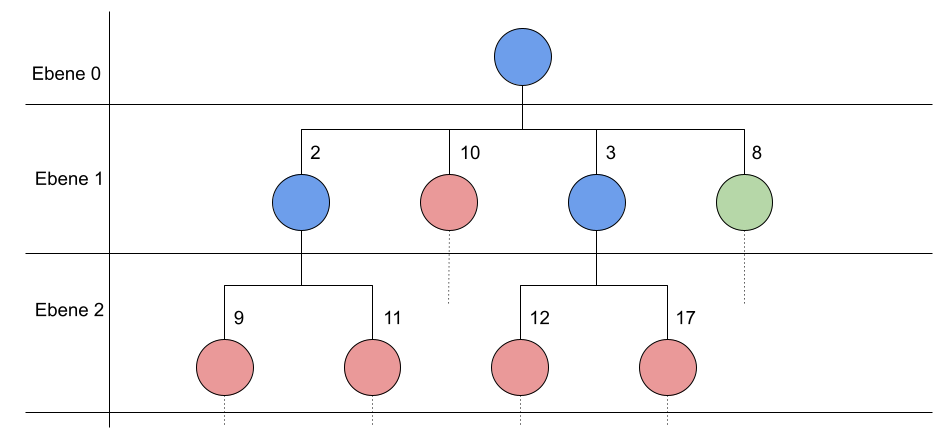
\includegraphics[width=0.8\linewidth]{../common/03_billiard_ai/resources/28_suchbaum_bewertung.png}
    \end{center}
    \caption{Bewertung eines Suchbaums: Die Knoten werden je nach Bedeutung mit unterschiedlichen Farben markiert.
    Wenn sie bereits expandiert wurden, sind sie blau. Grün, wenn der Knoten im nächsten Schritt expandiert wird,
    da er die geringsten Pfadkosten aufweist und rot, wenn der Knoten nicht in Frage kommt aufgrund zu hoher Kosten.}
    \label{fig:suchbaum_bewertung}
\end{figure}

Die Kosten werden auf Basis dreier Kriterien\footnote{Die Kriterien Distanz und Winkel werden wie
in Publikation \cite{inproceedings:billiard_ai:1} verwendet.} gebildet:
\begin{enumerate}
    \item Die \emph{Distanz}, welche eine Kugel zurücklegt.
    \item Der \emph{Winkel}, in welcher ein Zielpunkt getroffen werden muss.
    \item Die \emph{Indirektion}, wenn eine Kugel über die Banden oder über eine andere Kugel angestossen wird.
\end{enumerate}

Jeder dieser Werte liegt zwischen $0$ und $1$.
Die ersten beiden Kriterien sind in Abbildung \ref{fig:suche_knoten_expansionskosten} dargestellt.
Es werden zwei Expansionen gezeigt.
Die relevanten Informationen $d$ für die Distanz sowie $\alpha$ für den Winkel weisen
einen entsprechenden Index auf, welcher den Expansionsschritt markiert.
Beim ersten Expansionsschritt bildet der Zielpunkt
den Elternknoten.
Der Winkel $\alpha_1$ ist definiert durch die Rollrichtung der Kugel und einer Normalen auf den Zielpunkt.
Die Normalen zeigen jeweils zum Ursprung in der Mitte des Tisches.
Die Distanz $d_1$ ist definiert über die Länge des zurückzulegenden Weges.
Ist in einem Expansionsschritt die weisse Kugel betroffen, werden die Distanzkosten mit den
Distanzkosten des vorangegangenen Expansionsschritts gewichtet.
Dies stellt sicher, dass der Weg, welcher die nächste Kugel nehmen wird, möglichst kurz sein muss,
damit sich ein allfälliger Fehler beim Stoss der weissen Kugel nicht zu stark akkumuliert.
Im zweiten Fall wird der Winkel $\alpha_2$ durch die Rollrichtung der ersten und der Rollrichtung der zweiten Kugel definiert.

\begin{figure}[h!]
    \begin{center}
        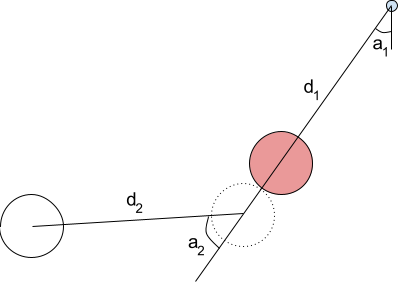
\includegraphics[width=0.4\linewidth]{../common/03_billiard_ai/resources/29_suchbaum_expansionskosten.png}
    \end{center}
    \caption{Zusammensetzung der Kosten eines Stosses:
    Die Kugeln müssen die Distanzen $d_1$ und $d_2$ zurücklegen.
    Die rote Kugel muss im Winkel $\alpha_1$ getroffen werden.
    Die rote Kugel wird dadurch im Winkel $\alpha_2$ in das Zielloch gespielt.
    Der Vektor $\vec{n}$ ist die Normale des Ziellochs, welche für die Berechnung des Winkels $\alpha_2$ verwendet wird.
    }
    \label{fig:suche_knoten_expansionskosten}
\end{figure}

Um die beiden Grössen vergleichen zu können, müssen sie in dieselbe Grössenordnung gebracht werden. Aus diesem Grund
werden sie durch die maximal möglichen Werte normiert \cite{qucosa:ein_billardroboter:1}. Für die Distanz ist dies die
Diagonale über den Tisch, für den Winkel wird ein maximal möglicher Wert von $87^\circ$ gewählt, dies ist bereits bei
der Suche berücksichtigt. Es gilt die Annahme, dass je kürzer der Weg und je kleiner der Winkel,
desto einfacher der Stoss.
\begin{align}
    d_{krit} = \frac{d_i}{d_{max}}\\
    \alpha_{krit} = \frac{\alpha}{\alpha_{max}}
\end{align}
Aktuell fliesst der Winkel $\alpha_{krit}$ zu stark in die Bewertung ein. Daher wird dieser durch eine kubische
Bézier-Kurve \cite{wiki.bezier:1} gewichtet. Die Parameter lauten wie folgt.
\begin{align}
    P_0 = \begin{pmatrix} 0 & 0\end{pmatrix}\\
    P_1 = \begin{pmatrix} 1 & 0\end{pmatrix}\\
    P_2 = \begin{pmatrix} 0.5 & 1\end{pmatrix}\\
    P_3 = \begin{pmatrix} 1 & 1\end{pmatrix}\\
    P = \begin{pmatrix} P_0 \\ P_1 \\ P_2 \\ P_3\end{pmatrix}\\
    T = \begin{pmatrix} t^3 & t^2 & t & 1\end{pmatrix}\\
    M = \begin{pmatrix}
            -1 &  3 & -3 & 1\\
             3 & -6 &  3 & 0\\
            -3 &  3 &  0 & 0\\
             1 &  0 &  0 & 0
        \end{pmatrix}\\
    \alpha^G_{krit} = f(t = \alpha_{krit}) = T \cdot M \cdot P
\end{align}
Nach dieser Gewichtung resultiert ein Punkt im zweidimensionalen Raum, wovon die y-Komponente als $\alpha^G_{krit, y}$ verwendet wird.
Die Kurve ist in Abbildung \ref{fig:suche_knoten_gewichtung_winkelkosten}
visualisiert. Es wird deutlich, dass kleinere Winkel einen eher geringen Einfluss auf die Kosten haben.
Ab einem Winkel von $50^\circ$, welcher auf der Grafik \ref{fig:suche_knoten_gewichtung_winkelkosten} als Punkt $D_1$ markiert ist,
beginnt die Kurve bis etwa $80^\circ$ stark zu steigen.
Ab dort flacht sie wiederum ab, bis die Kosten von $90^\circ$ schliesslich den Wert $1$ erreichen.

\begin{figure}[h!]
    \begin{center}
        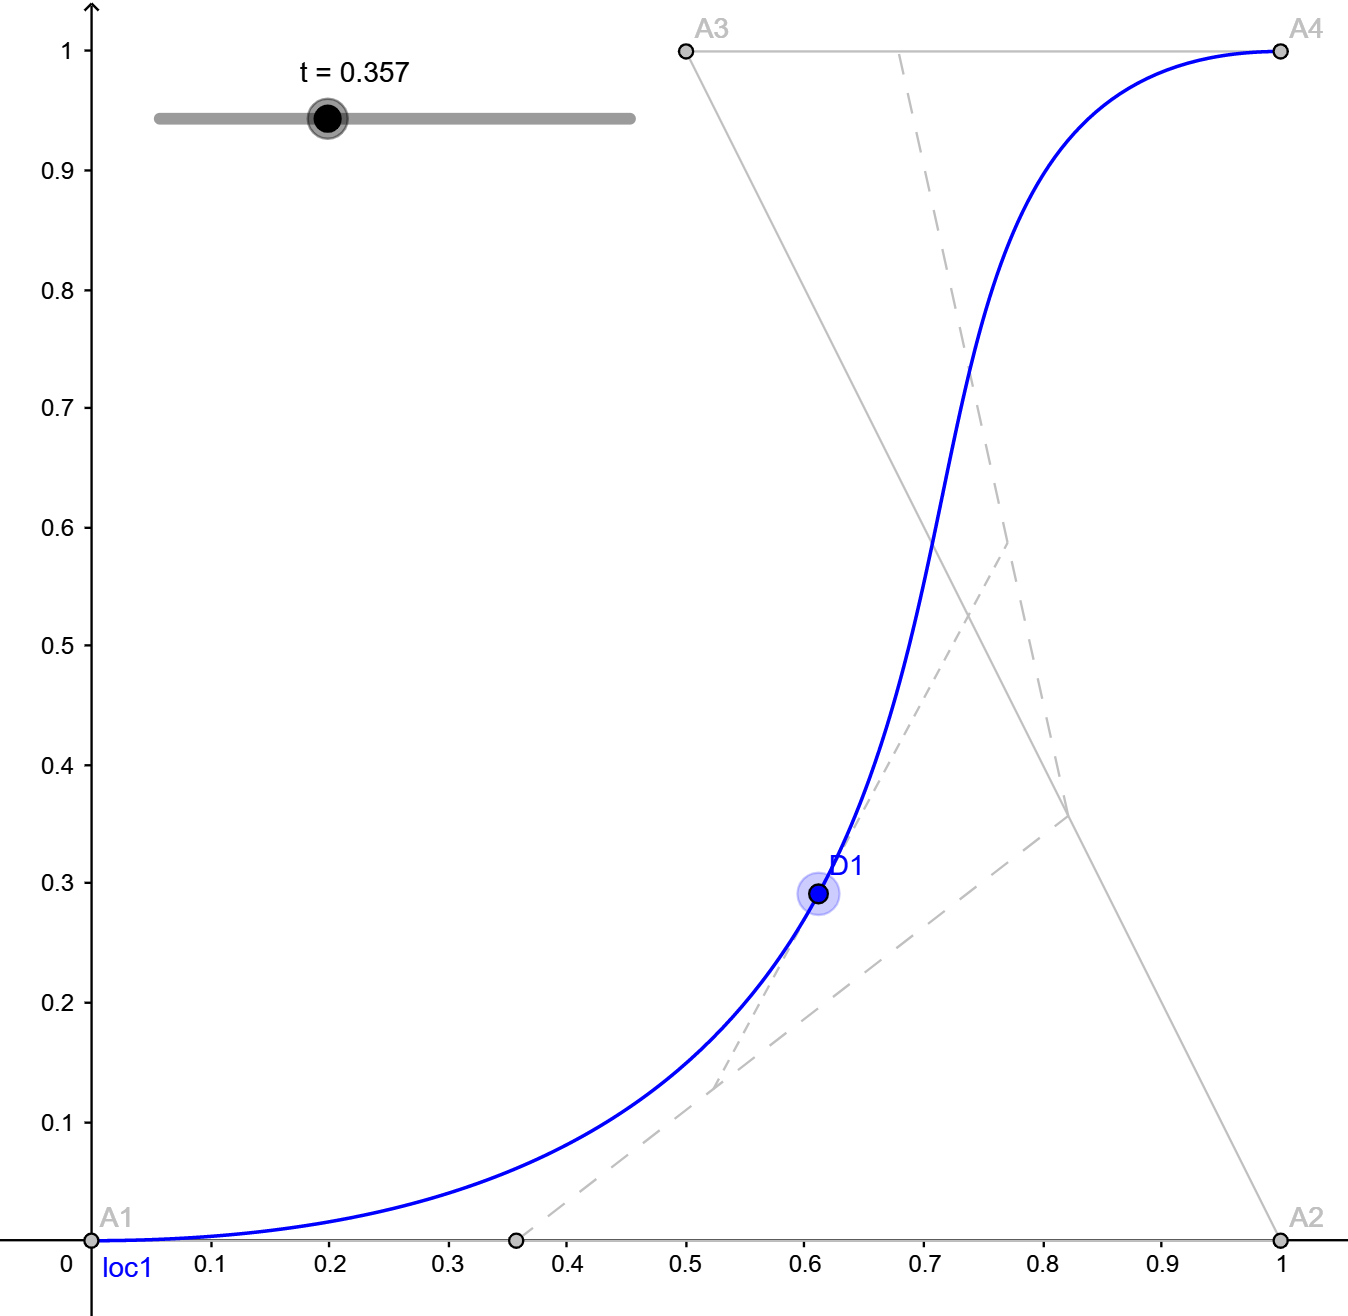
\includegraphics[width=0.4\linewidth]{../common/03_billiard_ai/resources/30_suchbaum_gewichtung_winkelkosten.png}
    \end{center}
    \caption{Gewichtung der Winkelkosten mittels einer Bézier-Kurve.
    Kleine Winkel werden in den Kosten geringer gewichtet, während grosse Winkel eine höhere Gewichtung erhalten.}
    \label{fig:suche_knoten_gewichtung_winkelkosten}
\end{figure}

Das Kriterium der Indirektion über Kugeln wird wiederum über einen maximal möglichen Wert gelöst.
Es wird eine maximale Indirektion $K_{I,max}$ angegeben und die Anzahl der Vorkommnisse ${K_{I,n}}$ wird durch die
Konstante dividiert. Dadurch werden die Kosten erhöht, je grösser der Indirektionsgrad ist.
\begin{align}
    K_{I,krit} = \frac{K_{I,n}}{K_{I,max}}
\end{align}

Das Kriterium der Indirektion über Banden wird ebenso über einen maximal möglichen Wert gelöst.
Es wird eine maximale Indirektion $K_{B,max}$ angegeben und die Anzahl der Vorkomnisse ${K_{B,n}}$ wird durch die
Konstante dividiert. Dadurch werden die Kosten erhöht, je grösser der Indirektionsgrad ist.
\begin{align}
    K_{B,krit} = \frac{K_{B,n}}{K_{B,max}}
\end{align}

Die endgültigen Kosten werden über die Addition aller Kriterien gebildet.
\begin{align}
    K = d_{krit} + \alpha^G_{krit, y} + K_{I,krit} + K_{B,krit}
\end{align}


\subsection{Berechnung der Initialgeschwindigkeit}\label{sec:initialgeschwindigkeit}
Sofern ein Stosskandidate wie in Abschnitt \ref{sec:kandidatensuche} beschrieben gefunden wurde, muss berechnet werden,
welche Geschwindigkeit die weisse Kugel erhalten muss, damit die gewünschte Kugel ins Loch gespielt wird.
Relevant dafür ist der Reibungsverlust wenn die Kugel rollt und die Kollision mit anderen Kugeln.

Wenn eine Kugel in ein Loch rollen soll, kann eine minimale Endgeschwindigkeit angenommen werden und aufgrund
der zurückzulegenden Strecke die Startgeschwindigkeit bestimmt werden, dies wird in Abschnitt \ref{ReibungsverlustUeberBahn} beschrieben.
Sofern diese Kugel über den Spielball ins Loch gespielt werden soll, dann muss der Spielball mit einer gewissen
Geschwindigkeit die Kugel treffen, damit diese die gewünschte Startgeschwindigkeit erhält. Dies wird in Abschnitt \ref{EnergieuebergabeBeiKollision} beschrieben.

\subsubsection{Reibungsverlust über Bahn}\label{ReibungsverlustUeberBahn}
Das Ziel eines Billiardstosses ist es, eine Kugel von einem Punkt A zu einem Punkt B rollen zu lassen.
Dabei findet Rollreibung statt, welche das Abbremsen der Kugel verursacht.
Es ist relevant zu wissen, welche Startgeschwindigkeit $v_1$ eine Kugel am Punkt A haben muss,
um mit der Endgeschwindigkeit $v_2$ am Punkt B anzukommen.
Beispielsweise wenn eine Kugel X in eines der Löcher gespielt werden soll,
wobei die Kugel eine gewisse minimale Endgeschwindigkeit haben soll, damit sie tatsächlich ins Loch rollt.

Es kann die nachfolgende Formel angewendet werden\footnote{Die Herleitung findet sich im Anhang \ref{anhang:herleitung:StartgeschwAnhandEndgeschwMitReibung}}:
\begin{align}
    \vec{v_1} = \sqrt{\norm{\vec{v_2}}^2 + 2 \cdot g \cdot c_R \cdot \Delta s} \cdot \frac{\vec{v_2}}{\norm{\vec{v_2}}}
\end{align}

Sei $S$ die Startposition der Kugel, $E$ die Endposition der Kugel und $V$ der gewünschte Betrag der Endgeschwindigkeit,
dann lässt sich die Endgeschwindigkeit $\vec{v_2}$ wie folgt berechnen:
\begin{align}
    \vec{\Delta s} = E - S\\
    \hat{\Delta s} = \frac{\vec{\Delta s}}{\norm{\vec{\Delta s}}}\\
    \vec{v_2} = V \cdot \hat{\Delta s}
\end{align}

\subsubsection{Elastischer Stoss bei Kugelkollision}\label{EnergieuebergabeBeiKollision}

Um eine Kugel T in eine gewünschte Richtung, wie etwa zum Loch, zu rollen, muss sie von einer anderen Kugel A,
evtl. vom Spielball, angestossen werden.
Es gilt herauszufinden, wo die Kugel T getroffen werden muss und welche Geschwindigkeit die Kugel A zum Kollisionszeitpunkt
haben muss, um die Kugel T in die gewünschte Richtung mit der geforderten Geschwindigkeit rollen zu lassen.

Die Situation mit der Kugel T, an der Position $C$ und der Kugel A, an der Position $A$ ist in Abbildung \ref{fig:ballCollisionPointReverse}
dargestellt. Die Kugel A muss zum Punkt $B$ rollen, wo sie auf Kugel T prallt und ein elastischer Stoss\cite{wiki.elastischer_stoss_physik:1} stattfindet.
Während die Kugel die Distanz $\norm{\vec{d}}$ zurücklegt, verliert sie an Geschwindigkeit aufgrund von Reibung,
diese wird in Abschnitt \ref{ReibungsverlustUeberBahn} behandelt. Hier ist lediglich relevant, welche Geschwindigkeit
die Kugel A am Punkt $B$ haben muss.

\begin{figure}[h!]
    \begin{center}
        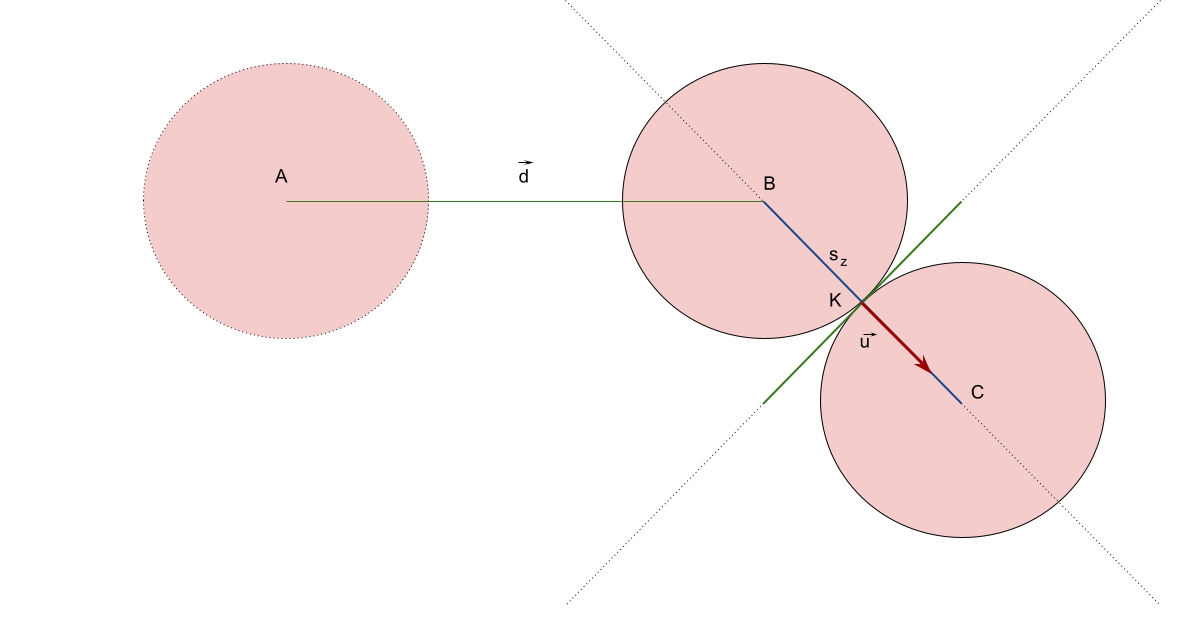
\includegraphics[width=0.6\linewidth]{../common/03_billiard_ai/resources/21_kollisionspunkt_rueckwaerts.png}
    \end{center}
    \caption{Kollisionspunkt zweier Kugeln}
    \label{fig:ballCollisionPointReverse}
\end{figure}

Sei $\vec{u}$, die gewünschte Richtung und Geschwindigkeit der Kugel T nach der Kollision,
dann ist der Zielpunkt $B$ der Kugel A wie folgt definiert\footnote{Die Herleitung findet sich im Anhang \ref{anhang:herleitung:ballCollisionReverse}}:
\begin{align}
    B = C - 2 \cdot r \cdot \hat{u}
\end{align}

Sei $\hat{d}$ der Richtungsvektor der Länge $1$ zwischen den Punkten $A$ und $B$, $E_v$ die Energieverlustkonstante in
Prozent, dann gilt für die Geschwindigkeit $\vec{v_1}$ der Kugel A bei der Kollision\footnote{Die Herleitung findet sich im Anhang \ref{anhang:herleitung:ballCollisionReverse}}:
\begin{align}
    \hat{u} = \frac{\vec{u}}{\norm{\vec{u}}}\\
    \vec{v_1} = \frac{\vec{u} \cdot \vec{u}}{\hat{d} \cdot \vec{u}} \cdot (1 + E_v) \cdot \hat{d}
\end{align}

Anschliessend kann die Startgeschwindigkeit der Kugel A an der Position A berechnet werden, weil die gewünschte
Endgeschwindigkeit und der zurückzulegende Weg bekannt ist\footnote{siehe Kapitel \ref{ReibungsverlustUeberBahn}}.

\newpage
\subsection{Modellierung physikalisches System}\label{kap:physikalisches_system}
Ein Stoss kann für die Simulation mithilfe eines Modells beschrieben werden.
Dieses Modell beschreibt den Ablauf eines Stosses durch Ereignisse, welche den beteiligten Objekten wiederfahren.
Die Kugeln, Banden und Löcher sind die Objekte dieses Modells.
Jedes Objekt dieses Modells hat einen veränderlichen Energiewert, bspw. sind Kugeln in Bewegung oder sie sind ruhend.
Eine Bande oder ein Loch bewegen sich nie, d.h. deren Energiewert ist konstant 0.
Kollisionen zweier Kugeln oder einer Kugel und der Bande sind Beispiele von Ereignissen, welche Veränderungen
der Energiezustände der Objekte bewirken.

Objekte, die einen Energiewert besitzen, welcher sich über die Zeit oder durch Interaktionen mit anderen Objekten verändert,
werden nachfolgend variabel genannt. Sofern ein variables Objekt einen Energiewert grösser 0 hat,
dann wird es weiter als dynamisch bezeichnet. Sobald es den Energiewert 0 erreicht, ist es als statisches
variables Objekt kategorisiert.
Banden und Löcher, welche einen fixen Energiewert besitzen, werden als konstant beschrieben.

Zwischen den Ereignissen kann eine Energieabnahme stattfinden. Beispielsweise unterliegt eine rollende Kugel der
Rollreibung und verliert dadurch bis zum nächsten Ereignis Energie.
Diese Energieabnahme erfolgt durch die Anwendung der Kantenfunktion auf der Kante zwischen zwei Ereignissen.

Diese Nomenklatur ist in Abbildung \ref{fig:physical_model_object_categories} ersichtlich.

\begin{figure}[h!]
    \begin{center}
        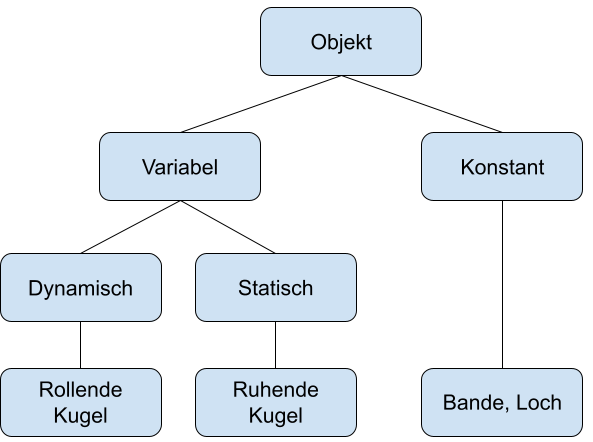
\includegraphics[width=0.5\linewidth]{../common/03_billiard_ai/resources/17_physical_model_categories.png}
    \end{center}
    \caption{Typen von Objekten}
    \label{fig:physical_model_object_categories}
\end{figure}

\newpage
\subsubsection{Ereignisse und ihre Repräsentation}
Das Ziel ist der Aufbau eines graphenähnlichen Konstrukts, welches aus Layern besteht und Zustandsübergänge variabler
Objekte durch Knoten repräsentiert.
Einige dieser Knoten treten bei Ereignissen wie einer Kollision oder wenn eine Kugel in ein Loch rollt auf.
Andere Knoten dienen der reinen Abbildung des variablen Objekts innerhalb des Layers.
Nachfolgend werden die Knoten definiert.

\begin{minipage}[t]{0.2\textwidth}
    \begin{center}
        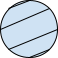
\includegraphics[width=0.3\linewidth]{../common/03_billiard_ai/resources/04_energy_input_node.png}
    \end{center}
\end{minipage}\hfill
\begin{minipage}[t]{0.8\textwidth}
    \textbf{Energy-Input-Node}: Dieser Node beschreibt das Auftreten eines Energie-Inputs von Aussen.
    Beispielsweise wenn die weisse Kugel mit dem Queue gestossen wird.
\end{minipage}\vskip.2\baselineskip
\begin{minipage}[t]{0.2\textwidth}
    \begin{center}
        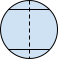
\includegraphics[width=0.3\linewidth]{../common/03_billiard_ai/resources/05_energy_transfer_node.png}
    \end{center}
\end{minipage}\hfill
\begin{minipage}[t]{0.8\textwidth}
    \textbf{Energy-Transfer-Node (Collision-Node)}: Dieser Node beschreibt die Übergabe von Energie auf die
    beteiligten Objekte. Ein Beispiel ist die Kollision zweier Kugeln, wobei diese Energie austauschen.
\end{minipage}\vskip.2\baselineskip
Der Energy-Transfer-Node wird in drei Schichten aufgeteilt. Bei der Input-Schicht wird die Kantenfunktion (siehe S. \pageref{cust:Kantenfunktion})
angewendet. Diese berücksichtigt den Energieverlust bis zum Auftreten des Ereignisses. Die mittlere Schicht beschreibt
die Übergabefunktion der beteiligten Objekte. Die dritte Schicht repräsentiert das Resultat, also den Status der
Objekte nach der Energieübergabe.
\begin{figure}[h!]
    \begin{center}
        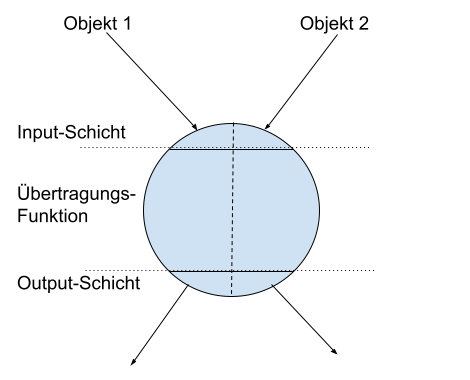
\includegraphics[width=0.5\linewidth]{../common/03_billiard_ai/resources/09_collision_node_description.png}
    \end{center}
    \caption{Der Energy-Transfer-Node}
    \label{fig:Der Energy-Transfer-Node}
\end{figure}\\
\begin{minipage}[t]{0.2\textwidth}
    \begin{center}
        
\includegraphics[width=0.3\linewidth]{../common/03_billiard_ai/resources/06_no_energy_node.png}
    \end{center}
\end{minipage}\hfill
\begin{minipage}[t]{0.8\textwidth}
    \textbf{No-Energy-Node}: Dieser Node wird eingesetzt, sobald der Energiewert eines variablen Objekts auf 0 sinkt und
    somit auch den Übergang von dynamisch zu statisch repräsentiert.
\end{minipage}\vskip.2\baselineskip
\begin{minipage}[t]{0.2\textwidth}
    \begin{center}
        
\includegraphics[width=0.3\linewidth]{../common/03_billiard_ai/resources/07_out_of_system_node.png}
    \end{center}
\end{minipage}\hfill
\begin{minipage}[t]{0.8\textwidth}
    \textbf{Out-Of-System-Node}: Dieser Node wird eingesetzt, sobald ein variables Objekt das System verlässt,
    indem beispielsweise eine Kugel in ein Loch rollt.
\end{minipage}\vskip.2\baselineskip
\begin{minipage}[t]{0.2\textwidth}
    \begin{center}
        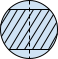
\includegraphics[width=0.3\linewidth]{../common/03_billiard_ai/resources/08_cutting_node.png}
    \end{center}
\end{minipage}\hfill
\begin{minipage}[t]{0.8\textwidth}
    \textbf{Cutting-Node}: Dieser Node ist ein spezieller Energy-Transfer-Node. Er wird bei variablen Objekten
    eingesetzt, die nicht an einem Ereignis beteiligt sind, wenn ein solches auftritt. Zum Ereigniszeitpunkt wird
    ein neuer Layer (siehe S. \pageref{cust:Layer}) geschaffen, welcher die Objekte, die am Ereignis beteiligt sind,
    in einem Energy-Transfer-Node festhält. Weiterhin wird der Status aller dynamsichen Objekte ebenfalls zu diesem
    Zeitpunkt festgehalten. Der Cutting-Node beschränkt sich auf ein Input- sowie Output-Objekt und beinhaltet als
    Energieübertragungsfunktion die Identitätsfunktion.
\end{minipage}\vskip.2\baselineskip

\subsubsection{Kantenfunktion} \label{cust:Kantenfunktion}
Die Kantenfunktion beschreibt eine Energieabnahme über die Zeit oder den Weg.

\subsubsection{Layer} \label{cust:Layer}
Ein Layer beinhaltet sämtliche Veränderungen der variablen Objekte und beschreibt den Status aller Objekte zu diesem Zeitpunkt.
Sobald ein Ereignis auftritt wird ein neuer Layer im Modell eingefügt.

\subsubsection{Beispiel eines Graphen}
Das beschriebene Datenmodell kann als Graph\footnote{Aus effizientsgründen wird auf einen Graphen in der Implementation
verzichtet. Das Modell setzt sich aus verschiedenen Layern zusammen, bei welchen die Informationen der Events für jedes
variable Objekt separat und mit Zugriffszeit $O(1)$ abgelegt werden.} visualisiert werden. Als Beispiel wird die Idee
eines Billardstosses in Abbildung \ref{fig:Beispiel für ein Resultat des Algorithmus phys_sys} hinzugezogen.
Auf dem Tisch liegt eine weisse wie auch zwei rote Kugeln. Die zweite rote Kugel wird an keiner Interaktion beteiligt sein,
weswegen sie ihren Zustand nie verändert. Es ist ersichtlich, dass bei jedem Ereignis für diese Kugel ein \glqq Out-of-energy-Node\grqq{}
eingefügt wird.
Das erste Event beschreibt die Kollision des dynamischen Objekts \glqq weisse Kugel\grqq{} sowie des
statischen Objekts \glqq rote Kugel\grqq{}. Danach verliert die weisse Kugel sämtliche Energie und wechselt in den
Status \glqq Out-of-energy\grqq{}. Da die rote Kugel zu diesem Zeitpunkt dynamisch ist, wird für sie ein
\glqq Cutting-Node\grqq{} eingefügt. Zuletzt rollt die rote Kugel in das Loch, für sie wird ein \glqq Out-of-system-Node\grqq{}
erstellt und das System hat sämtliche Energie verloren. Ein Endzustand wurde erreicht, da alle Kugeln nun statisch sind.

\begin{figure}[h!]
    \begin{center}
        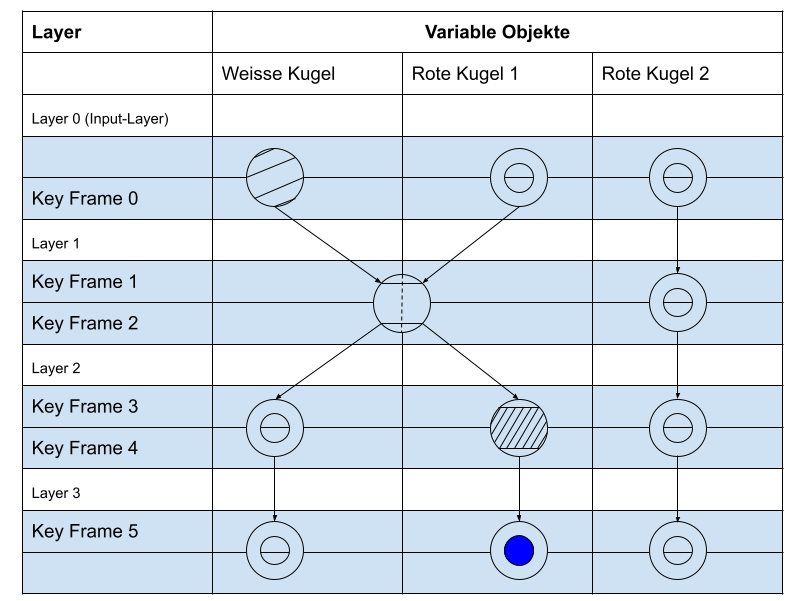
\includegraphics[width=0.6\linewidth]{../common/03_billiard_ai/resources/10_datenmodell_beispiel.png}
    \end{center}
    \caption{Beispiel für ein Resultat des Algorithmus \ref{alg:physikalisches_system}}
    \label{fig:Beispiel für ein Resultat des Algorithmus phys_sys}
\end{figure}

In Algorithmus \ref{alg:physikalisches_system} wird die Grundidee erläutert. Als Input für die Funktion \glqq simulate\grqq{}
dient der erste Layer, welcher mehrere variable Objekte beinhalten kann, wobei mindestens ein Objekt dynamisch (energiereich)
sein sollte. Dieser Layer wird direkt dem erzeugten System hinzugefügt und dieses wird solange bearbeitet, bis alle variablen
Objekte statisch sind (das System hat keine Energie mehr). In jedem Schleifendurchlauf wird das nächste Event berechnet.
Die Events können diverser Natur sein. Es werden Kollisionen mit dynamischen, statischen wie auch konstanten Objekten
geprüft. Bei der Kollision mit konstanten Objekten können die Ereignisse \glqq Energy transfer\grqq{} oder \glqq Out of
System\grqq{} auftreten. Weiterhin wird geprüft, ob ein dynamisches Objekt seine Energie durch die Kantenfunktion
verliert.
Aufgrund eines Ereignisses wird zunächst ein neuer Layer generiert, dann für die am Ereignis beteiligten Objekte
den entsprechenden Node und zuletzt für die anderen variablen Objekte entweder ein \glqq Cutting-Node\grqq{} oder ein
\glqq Out-of-energy-Node\grqq{} eingefügt.

\begin{algorithm}[H]
    \DontPrintSemicolon
    \SetKwFunction{simulate}{simulate}
    \SetKwFunction{nextEvent}{nextEvent}
    \SetKwFunction{atMoment}{atMoment}
    \SetKwProg{Fn}{Function}{}{}
    \Struct{Event}{
        timestamp: datetime\\
        me: string\\
        partner: string\\
        partnerType: [BALL, TARGET, RAIL]\\
        event: [OutOfEnergy, Collision]\\
    }
    \;
    \Fn{\simulate{start: Layer, constantObjects: list} $\longrightarrow$ System}{
        system $\longleftarrow$ System()\\
        system $\longleftarrow$ appendLayer(system, start)\\
        \While{! system.isStatic()}{
            nextEvent $\longleftarrow$ nextEvent(system.lastLayer(), constantObjects)\\
            layer $\longleftarrow$ atMoment(system.lastLayer(), nextEvent)\\
            system $\longleftarrow$ appendLayer(system, start)
        }
        \KwRet system
    }
    \;
    \Fn{\nextEvent{layer: Layer, constantObjects: list} $\longrightarrow$ Event}{
        nextEvent: Event $\longleftarrow$ none\\
        \For{object in layer.dynamicObjects()}{
            nextEvent $\longleftarrow$ min(nextEvent, outOfEnergy(object))\\
            nextEvent $\longleftarrow$ min(nextEvent, collision(object, layer.dynamicObjects()))\\
            nextEvent $\longleftarrow$ min(nextEvent, collision(object, layer.staticObjects()))\\
            nextEvent $\longleftarrow$ min(nextEvent, collision(object, constantObjects))
        }
        \KwRet nextEvent
    }
    \;
    \Fn{\atMoment{layer: Layer, event: Event} $\longrightarrow$ Event}{
        nextLayer $\longleftarrow$ layer()
        \For{node in layer.objects()}{
            \If{node.first == event.me or node.first == event.partner}{
                nextLayer $\longleftarrow$ append(nodeForEvent(node, event))
            }
            \Else{
                \If{node.second.hasEnergy()}{
                    nextLayer $\longleftarrow$ append(cuttingNode(node, event.timestamp))
                }\Else{
                    nextLayer $\longleftarrow$ append(node, nextLayer)
                }
            }
        }
        \KwRet nextLayer
    }
    \caption{Algorithmus zum Aufbau eines physikalischen Systems}
    \label{alg:physikalisches_system}
\end{algorithm}


\subsection{Simulation}\label{kap:simulation}
Sobald ein möglicher Lösungskandidat anhand der in Abschnitt \ref{sec:kandidatensuche} beschriebenen Suche gefunden
und dessen Initialgeschwindigkeit nach Abschnitt \ref{sec:initialgeschwindigkeit} berechnet wurde,
wird eine Simulation durchgeführt, um die Lösung definitiv zu bestätigen.
Durch das Anwenden verschiedener Anfangsgeschwindigkeiten der weissen Kugel können in diesem Schritt mehrere Situationen evaluiert werden.

Die Simulation wird durch die Definition eines physikalischen Systems wie in Kapitel \ref{kap:physikalisches_system} durchgeführt.
Hierbei gelten die Zuordnungen wie sie nachfolgend beschrieben werden.\\
\textbf{Ereignisse}
\begin{description}
    \item[Energy-Input-Node] Wird modelliert über die Eingabe der Energie der weissen Kugel. Ein spezifischer Node zur
    Modellierung wird nicht implementiert, es wird der Energy-Transfer-Node verwendet, wobei nur der Output-Wert relevant ist.
    \item[Energy-Transfer-Node] Tritt bei der Kollision zwischen zwei Kugeln oder einer Kugel mit der Bande auf.
    \item[No-Energy-Node] Tritt auf, wenn eine Kugel vom dynamischen in den statischen Zustand wechselt (ausrollt). In jedem
    Layer, wo eine Kugel statisch ist, wird sie durch diesen Node modelliert.
    \item[Out-of-System-Node] Sobald eine Kugel mit dem Zielkreis kollidiert, tritt dieses Ereignis auf. Dem System wird die
    Energie entzogen und die Kugel ist nicht mehr verfügbar.
\end{description}

\textbf{Kantenfunktion}
Die Kantenfunktion zwischen den Übergängen innerhalb des Layers bildet der Reibungsverlust der
Kugel über eine bestimmte Zeit oder einen bestimmten Ort.

\textbf{Dynamische/Statische Objekte}
Im Billiard gibt es nur die Kugeln als statische und/oder dynamische Objekte.

\textbf{Konstante Objekte}
Die konstanten Objekte bilden die Banden wie auch die Ziele.

Es wird ungefähr der Pseudoalgorithmus wie in \ref{alg:physikalisches_system} angewendet, optimal auf das Problem \glqq{}Billiard\grqq{}
abgestimmt. Es folgen die physikalischen Berechnungen zur Durchführung der Simulation.


\subsubsection{Reibungsverlust über die Zeit}
Die Geschwindigkeit einer Kugel wird durch die Reibung über die Zeit reduziert. Dazu wird die Formel der gleichförmig
beschleunigten Bewegung verwendet, wobei $\vec{v_0}$, $\vec{a}$ sowie $t$ gegeben sind.
\begin{align}
    \vec{v} = \vec{a} \cdot t + \vec{v_0}
\end{align}

\subsubsection{Elastischer Stoss zweier Kugeln}\label{kap:simulation:elastischer_stoss_zweier_kugeln}
Die Kollision zweier Kugeln wird im Folgenden als zweidimensionaler elastischer Stoss angesehen. Dabei ist es wichtig,
zwei Komponenten beim Zusammenprall zu betrachten. Dies ist einerseits das Liniensegment $s_z$ zwischen den Mittelpunkten
der Kugeln sowie die orthogonal dazu stehende Gerade $s_t$. Die Kugel, welche Energie mitbringt, übergibt der anderen
Kugel Energie in Richtung von $s_z$. Die übrig gebliebene Energie zeigt in Richtung von $s_t$ \cite{wiki.elastischer_stoss_physik:1}.
In Abbildung \ref{fig:Elastischer Stoss zweier Kugeln} ist ein solcher Stoss dargestellt.
Kugel eins bringt dabei die Geschwindigkeit $\vec{v_1}$ und Kugel zwei die Geschwindigkeit $\vec{v_2}$ mit. Ein Anteil
der Geschwindigkeit von Kugel eins wird der Kugel zwei in Richtung von $s_z$ übergeben. Dasselbe gilt für die
Kugel zwei. Sie übergibt einen Teil ihrer Geschwindigkeit an Kugel eins ebenfalls in Richtung von $s_z$. Die verbleibende
Energie der Kugeln zeigt jeweils in Richtung von $s_t$.
\begin{figure}[h!]
    \begin{center}
        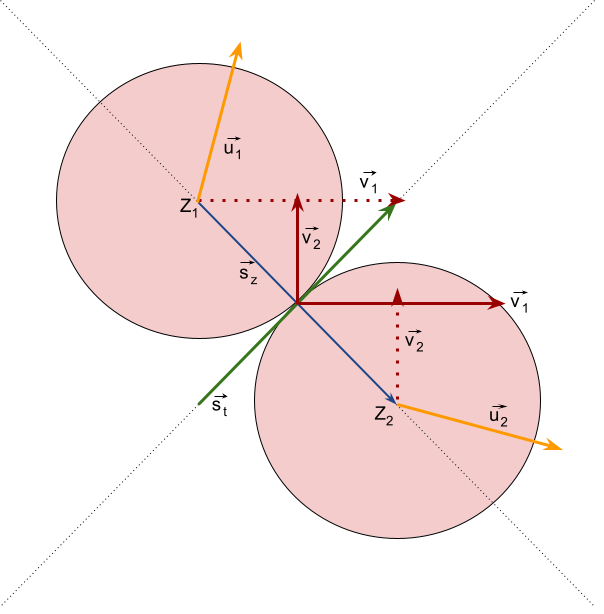
\includegraphics[width=0.4\linewidth]{../common/03_billiard_ai/resources/23_elastischer_stoss.png}
    \end{center}
    \caption{Elastischer Stoss zweier Kugeln}
    \label{fig:Elastischer Stoss zweier Kugeln}
\end{figure}

Die initialen Geschwindigkeiten $\vec{v^i_1}$ und $\vec{v^i_2}$ werden aufgrund eines Energieverlusts um eine
Konstante $E_v$, welche in Prozent angegeben wird, reduziert. Dies ist notwendig, da in der Realität durch Reibung
die Energie nicht vollständig weitergegeben wird.
\begin{align}
    \vec{v_1} = \vec{v^i_1} \cdot (1 - E_v)\\
    \vec{v_2} = \vec{v^i_2} \cdot (1 - E_v)\\
\end{align}
Um nun die neuen Geschwindigkeiten $\vec{u_1}$ und $\vec{u_2}$ zu berechnen, müssen die initialen Geschwindigkeiten
$\vec{v_1}$ sowie $\vec{v_2}$ auf die Komponenten in Richtung von $s_z$ und $s_t$ aufgeteilt werden.
\begin{align}
    \vec{z} = \vec{Z_2} - \vec{Z_1}\\
    \hat{z} = \frac{\vec{z}}{\norm{\vec{z}}}
\end{align}
Von Interesse ist dabei nur $\hat{z}$.
Mit diesem Vektor kann die Komponente in Richtung $s_z$ beider Geschwindigkeiten ermittelt werden.
\begin{align}
    \vec{v_{1,z}} = (\vec{v_1} \cdot \hat{z}) \cdot \hat{z}\\
    \vec{v_{2,z}} = (\vec{v_2} \cdot \hat{z}) \cdot \hat{z}
\end{align}
Mittels dieses neuen Vektors in Richtung $s_z$ kann der Vektor in Richtung $s_t$ berechnet werden.
\begin{align}
    \vec{v} = \vec{v_t} + \vec{v_z}\\
    \vec{v_t} = \vec{v} - \vec{v_z}
\end{align}
Daraus folgt für die jeweiligen Kugeln:
\begin{align}
    \vec{v_{1,t}} = \vec{v_1} - \vec{v_{1,z}}\\
    \vec{v_{2,t}} = \vec{v_2} - \vec{v_{2,z}}
\end{align}
Die neuen Geschwindigkeitsvektoren setzen sich wie beschrieben aus den jeweiligen Komponenten zusammen.
Das Resultat lautet wie folgt:
\begin{align}
    \vec{u_1} = \vec{v_{2,z}} + \vec{v_{1,t}}\\
    \vec{u_2} = \vec{v_{1,z}} + \vec{v_{2,t}}
\end{align}

\paragraph{Behandlung Rollverhalten} \hfill \\
Da eine Kugel nicht nur gleitet sondern auch rollt und kaum Reibung mit der kollidierenden Kugel hat, hat dieses Rollen im
Falle einer Kugelkollision einen Einfluss auf den weiteren Verlauf der vorher dynamischen Kugeln.
Es werden zwei Ansätze erläutert. Die erste Variante behandelt das Rollen als ablenkende Kraft in eingehender Richtung mit konstantem Betrag.
Die zweite Variante berücksichtigt zusätzlich die Variabilität des Rollens. In Abbildung \ref{fig:einfluss_rollen} wird der Einfluss des
Rollens bei grossen wie auch kleinen Geschwindigkeiten erläutert.

Bei Variante eins wird der Einfluss des Rollens berücksichtigt,
indem bei den vorher dynamischen Kugeln ein Vektor mit konstantem
Betrag in der einkommenden Geschwindigkeitsrichtung auf den durch die elastische Kollision berechneten Vektor
$\vec{v_{k,t}}$ aufaddiert wird. Demnach gilt für den neuen Vektor $\vec{v_{k,t,n}}$ der Kugeln, wobei $A$ für die konstante Geschwindigkeit und
$\hat{v_k}$ für den normierten Vektor $\vec{v_k}$ der Kugel $k$ steht.
\begin{align}
    \vec{v_{1,t,n}} = \vec{v_{1,t}} + A \cdot \hat{v_1}\\
    \vec{v_{2,t,n}} = \vec{v_{2,t}} + A \cdot \hat{v_2}
\end{align}

Dieser Vektor $\vec{v_{k,t,n}}$ wird nun anstelle von $\vec{v_{k,t}}$ verwendet, wobei die maximale Energie des Vektors
auf die Eingangsenergie beschränkt wird.
\begin{align}
    \vec{u_1} = \vec{v_{2,z}} + \min{(\vec{v_{1,t,n}}, \norm{\vec{v_1}} \cdot \hat{{v_{1,t,n}}})}\\
    \vec{u_2} = \vec{v_{1,z}} + \min{(\vec{v_{2,t,n}}, \norm{\vec{v_2}} \cdot \hat{v_{2,t,n}})}
\end{align}

\begin{figure}[h!]
    \centering
    \begin{subfigure}[b]{0.6\textwidth}
        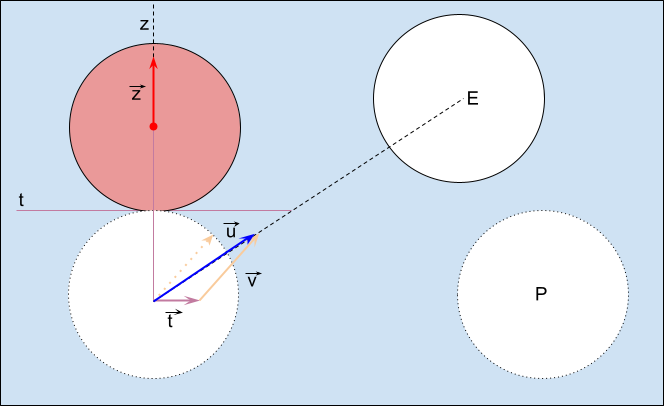
\includegraphics[width=1\textwidth]{../common/03_billiard_ai/resources/33_rollen_kleine_geschwindigkeit.png}
        \caption{Rolleinfluss bei kleiner Geschwindigkeit}
        \label{fig:rollen_kleine_geschwindigkeit}
    \end{subfigure}\\
    \begin{subfigure}[b]{0.6\textwidth}
        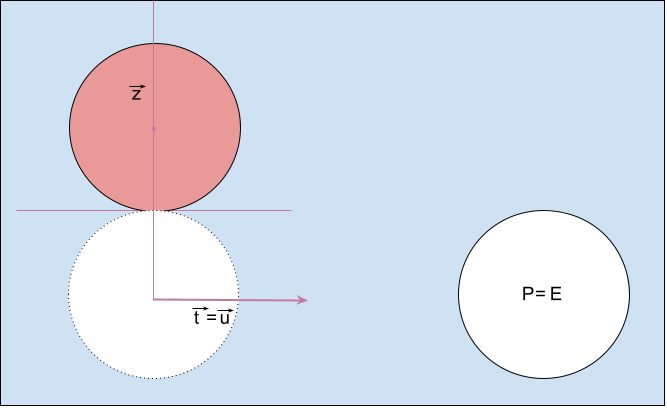
\includegraphics[width=1\textwidth]{../common/03_billiard_ai/resources/34_gleiten_grosse_geschwindigkeit.png}
        \caption{Kein Rollen bei grosser Geschwindigkeit}
        \label{fig:gleiten_grosse_geschwindigkeit}
    \end{subfigure}
    \caption{(a) Eine einkommende Geschwindigkeit $\vec{v}$ wird auf die Komponenten $\vec{z}$ und $\vec{t}$ nach dem
    elastischen Stoss aus Kapitel \ref{kap:simulation:elastischer_stoss_zweier_kugeln} aufgeteilt.
    Ohne Berücksichtigung des Rollens wird die Position der weissen Kugel bei $P$ berechnet, die effektive Position ist bei $E$.
        (b) Bei grösserer Geschwindigkeit fängt die Kugel erst später an zu rollen. Zum Kollisionszeitpunkt gleitet sie
        in diesem Fall nur und es gilt der zweidimensionale elastische Stoss wie in
        Kapitel \ref{kap:simulation:elastischer_stoss_zweier_kugeln} beschrieben.
        $P$ und $E$ stimmen in diesem Fall überein.}
    \label{fig:einfluss_rollen}
\end{figure}

Variante zwei verfolgt einen ähnlichen Ansatz, jedoch wird bei der Berechnung von $\vec{v_{k,t,n}}$ anstelle des normierten
der initiale Geschwindigkeitsvektor verwendet, welcher mit einem Prozentsatz skaliert wird. Dadurch wird die Variabilität
berücksichtigt. Es gilt, dass $A$ zwischen $0$ und $1$ liegt.
\begin{align}
    \vec{v_{1,t,n}} = \vec{v_{1,t}} + A \cdot \vec{v_1}\\
    \vec{v_{2,t,n}} = \vec{v_{2,t}} + A \cdot \vec{v_2}
\end{align}

Die Berechnung von $\vec{u_1}$ sowie $\vec{u_2}$ geschieht auf dieselbe Art und Weise wie bei Variante eins.
Implementiert wurde die zweite Variante, da die variable Rollenergie dadurch mitberücksichtigt wird.

\newpage
\subsubsection{Bandenreflektion}
Sofern eine Kugel an eine Bande stösst, wird diese abgelenkt. In dem hier beschriebenen Modell wird der Drall\cite{wiki.spin:1},
welcher die Bahn einer Kugel nach Kollision mit der Bande ablenken würde, ignoriert.
Das bedeutet, es wird davon ausgegangen, dass der Ausfallswinkel nach der Bandenreflektion gleich dem Einfallswinkel sei.
Dazu kann die folgende Formel\cite{paulbourke.reflected_ray:1} verwendet werden, wobei $I$ der einfallende
und $R$ der ausgehende Weg der Kugel und $N$ der Normalenvektor der Bande sind:
\begin{align}
    R = I - 2 \cdot N \cdot (I \cdot N)
\end{align}

Da bei einer Bandenkollision Energie verloren geht, wird dieses Verhalten mit der Konstanten $E_v$ modelliert.
Diese gibt den Verlust in Prozent an.
\begin{align}
    R = (I - 2 \cdot N \cdot (I \cdot N)) \cdot \frac{1}{1 + E_v}
\end{align}
\subsubsection{Kollisionsprüfung}
Während der Simulation ist es notwendig zu prüfen, welche Kugeln mit welchen kollidieren könnten.
Um zu wissen, ob eine Kugel eine Strecke zurücklegen kann, ohne mit einer anderen Kugel zu kollidieren,
muss für jede andere Kugel geprüft werden, ob diese im Weg liegt. Daher sollte dieser Test effizient sein.
Für den Test wird die zurückzulegende Strecke als Liniensegment zwischen Punkt $A$ und Punkt $B$ und die Position
einer zu testenden Kugel $C$ als Punkt verstanden. Anschliessend wird der Abstand zwischen dem Punkt $C$ und dem
Liniensegment $AB$ geprüft, ob dieser kleiner als der Kugeldurchmesser ist. Sofern dies der Fall ist, liegt die Kugel an
der Position $C$ im Weg und es würde eine Kollision stattfinden, sofern die Ausgangskugel die Strecke $AB$ rollt.
Dies wird für jede Kugel geprüft.

\subsubsection{Ereignis - Energie-Transfer über Kugelkollision}
Dieses Ereignis beschreibt die Kollision mit einer anderen Kugel zum Zeitpunkt $t$.
Bekannt sind dabei die Beschleunigung $\vec{a}$\footnote{Die Beschleunigung $\vec{a}$ ist durch die Herleitung in Kapitel \ref{anhang:herleitung:beschleunigung}
gegeben.}, die Geschwindigkeit $\vec{v}$ und der Ort $\vec{s}$ beider Kugeln.
Diese werden entsprechend indexiert.

Weiterhin sind folgende Abstraktionen bekannt:
\begin{align}
    \vec{\Delta a} = \vec{\Delta a}_1 - \vec{\Delta a}_2\\
    \vec{\Delta v} = \vec{\Delta v}_1 - \vec{\Delta v}_2\\
    \vec{\Delta s} = \vec{\Delta s}_1 - \vec{\Delta s}_2
\end{align}

Es entsteht ein Polynom vierten Grades\footnote{Herleitung siehe Anhang \ref{anhang:herleitung:event:dynamicObjectCollision}}.
Um diese Gleichung zu lösen, bedarf es der entsprechenden Lösungsformel \cite{wiki.polynom:1}:
\begin{align}
    ax^4 + bx^3 + cx^2 + dx + e = 0\\
    x_{1,2} = -\frac{b}{4a} - S \pm \frac{1}{2}\sqrt{-4S^2 - 2p + \frac{q}{S}}\\
    x_{3,4} = -\frac{b}{4a} + S \pm \frac{1}{2}\sqrt{-4S^2 - 2p - \frac{q}{S}}\\
    p = \frac{8ac - 3b^2}{8a^2}\\
    q = \frac{b^3 - 4abc + 8a^{2}d}{8a^3}\\
    S = \frac{1}{2}\sqrt{-\frac{2}{3}p + \frac{1}{3a}(Q + \frac{\Delta_0}{Q})}\\
    Q = \sqrt[3]{\frac{\Delta_1 + \sqrt{\Delta_{1}^2 - 4\Delta_{0}^3}}{2}}\\
    \Delta_0 = c^2 - 3bd + 12ae\\
    \Delta_1 = 2c^3 - 9bcd + 27b^{2}e + 27ad^2 - 72ace
\end{align}

Wobei die Koeffizienten folgendermassen lauten:
\begin{align}
    a = \frac{1}{4} \cdot (\vec{\Delta a} \cdot \vec{\Delta a})\\
    b = \vec{\Delta a} \cdot \vec{\Delta v}\\
    c = \vec{\Delta a} \cdot \vec{\Delta s} + \vec{\Delta v} \cdot \vec{\Delta v}\\
    d = 2 \cdot (\vec{\Delta v} \cdot \vec{\Delta s})\\
    e = \vec{\Delta s} \cdot \vec{\Delta s} - D^2
\end{align}

Durch Lösen des Polynoms werden alle Zeitpunkte $x_{1-4} = t_{1-4}$ bestimmt, wobei der relevante Zeitpunkt $t$ der
Erste ist.
\begin{align}
    t = \min{(t_1, t_2, t_3, t_4)}
\end{align}

\paragraph{Performanceverbesserungen}\label{kap:kugelkollision:performanceverbesserung} \hfill \\
Das Lösen dieses Gleichungssystems erfordert viel Rechenzeit, was die Frage nach Performanceverbesserungen aufwirft.
Diese werden durch Vorbedingungen erzielt, welche geprüft werden. Es findet zu Beginn eine Fallunterscheidung
statt. Wenn die zweite Kugel statisch ist, so wird geprüft, ob die Distanz $d$ zwischen der Position $P_2$ der zweiten Kugel
$K_2$ und der halben Geraden $g$ definiert durch die Position $P_1$ der ersten Kugel $K_1$ wie auch deren Geschwindigkeitsvektor
$\vec{v}$ kleiner oder gleich dem Kugeldurchmesser ist. Nur in diesem Fall kann es eine Kollision geben.
Sämtliche Angaben beziehen sich auf die Grafik \ref{fig:kugelkollision_vorbedingung_statisch}.

\begin{figure}[h!]
    \begin{center}
        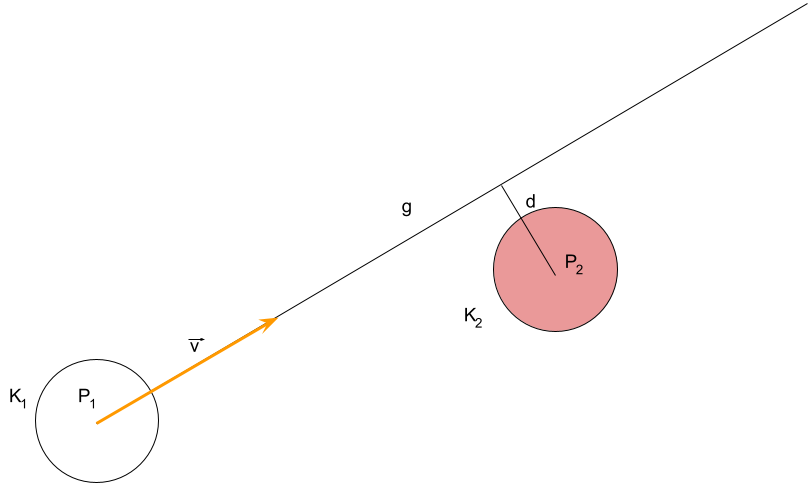
\includegraphics[width=0.4\linewidth]{../common/03_billiard_ai/resources/24_vorbedingung_kugelkollision_statisch.png}
    \end{center}
    \caption{Vorbedingung einer Prüfung auf Kollision zwischen Kugeln bei statischer Beteiligung}
    \label{fig:kugelkollision_vorbedingung_statisch}
\end{figure}

Sobald beide Kugeln dynamisch sind reicht eine einfache Prüfung auf die Distanz nicht mehr. Es muss ein Schnittpunkttest der beiden halben Geraden, definiert durch die
beiden Geschwindigkeitsvektoren, durchgeführt werden. Hierbei ist der Durchmesser der Kugel zu beachten, dies
wird in Abbildung \ref{fig:kugelkollision_vorbedingung_dynamisch} dargestellt.
\begin{figure}[h!]
    \begin{center}
        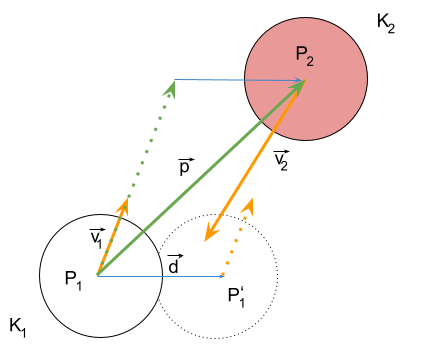
\includegraphics[width=0.4\linewidth]{../common/03_billiard_ai/resources/25_vorbedingung_kugelkollision_dynamisch.png}
    \end{center}
    \caption{Vorbedingung einer Prüfung auf Kollision zwischen dynamischen Kugeln}
    \label{fig:kugelkollision_vorbedingung_dynamisch}
\end{figure}

Daher wird der Vektor $\vec{p}$ zwischen den Positionen $P_1$ und $P_2$ gebildet (grün).
\begin{align}
    \vec{p} = P_2 - P_1
\end{align}
Der erhaltene Vektor wird auf den Geschwindigkeitsvektor $\vec{v_1}$ projiziert (grün gestrichelt).
\begin{align}
    \vec{p'} = (\vec{p} \cdot \hat{v_1}) \cdot \hat{v_1}
\end{align}
Danach wird der Zwischenvektor $\vec{d}$ gebildet (blau).
\begin{align}
    \vec{d} = \vec{p} - \vec{p'}
\end{align}

Die Kugel $K_1$ wird um diesen Vektor verschoben, es resultiert $P^{'}_1$.
\begin{align}
    P^{'}_1 = P_1 + \vec{d}
\end{align}
Von dieser Position aus kann nun ein Schnittpunkttest zwischen den beiden
halben Geraden, durch die Geschwindigkeitsvektoren definiert, durchgeführt werden.

Zudem gibt es zwei Spezialfälle zu beachten. Der erste beschreibt die Handhabung bei paralleler Fortbewegung
der Kugeln. Da dies ein sehr seltener Fall ist und
wohl kaum auftreten wird, wird die Berechnung zugelassen, wenn der Vektor $\vec{d}$ kleiner oder gleich gross
wie der Durchmesser ist. Die Situation wird in Abbildung \ref{fig:kugelkollision_vorbedingung_dynamisch_parallel} erläutert, die Berechnungen für den Vektor $\vec{d}$
sind äquivalent zu den vorhergehenden Berechnungen.
\begin{figure}[h!]
    \begin{center}
        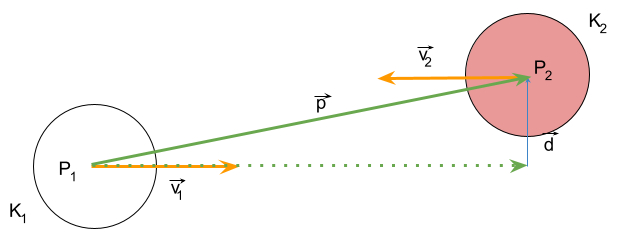
\includegraphics[width=0.4\linewidth]{../common/03_billiard_ai/resources/26_vorbedingung_kugelkollision_dynamisch_parallel.png}
    \end{center}
    \caption{Vorbedingung einer Prüfung auf Kollision zwischen dynamischen parallellaufenden Kugeln}
    \label{fig:kugelkollision_vorbedingung_dynamisch_parallel}
\end{figure}

Der letzte Spezialfall befasst sich mit der Tatsache, dass ein Schnittpunkttest, so wie er unter Berücksichtigung der
obigen Fälle durchgeführt wird, kein Ergebnis findet, wenn der Schnittpunkt hinter einer der Geraden liegt.
Diese Situation kann in Abbildung \ref{fig:kugelkollision_vorbedingung_dynamisch_hintereinander} entnommen werden.
Es ist ersichtlich, dass der Geschwindigkeitsvektor $\vec{v_1}$ einen grösseren Betrag aufweist als der
Geschwindigkeitsvektor $\vec{v_2}$. Um diesem Umstand Rechnung zu tragen, wird die Startposition der Geraden um den
Durchmesser nach hinten verschoben.
\begin{figure}[h!]
    \begin{center}
        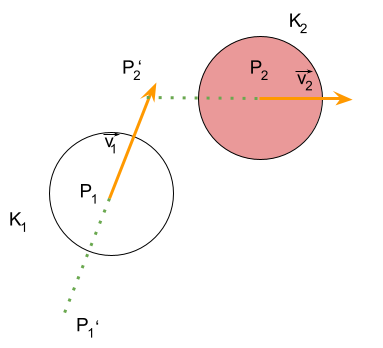
\includegraphics[width=0.4\linewidth]{../common/03_billiard_ai/resources/27_vorbedingung_kugelkollision_dynamisch_hintereinander.png}
    \end{center}
    \caption{Vorbedingung einer Prüfung auf Kollision zwischen dynamischen hintereinander verlaufenden Kugeln}
    \label{fig:kugelkollision_vorbedingung_dynamisch_hintereinander}
\end{figure}

\subsubsection{Ereignis - Energie-Transfer über Bandenkollision}
Dieses Event beschreibt die Kollision mit der Bande. Es soll der Zeitpunkt $t$ der Kollision mit der Bande festgestellt werden.
Der Algorithmus funktioniert so, dass zuerst geprüft wird, ob eine Kollision stattfinden kann.
Dies erfolgt über einen Schnittpunkt-Test zwischen einer Linie und einem Liniensegment.
Eine Bande kann als Liniensegment zwischen dem Startpunkt $R_1$ und $R_2$ betrachtet werden. Diese Punkte müssen demnach bekannt sein.
Weiterhin ist der Geschwindigkeitsvektor $\vec{v}$ und die Position der Kugel $C$ bekannt.
Aufgrund dieser Informationen kann eine Linie definiert werden.

Die Punkte $R_1$ und $R_2$ werden um den Kugelradius zur Tischmitte verschoben,
damit dem Kugelradius Rechnung getragen wird und dieser nicht weiter betrachtet werden muss.
Daraus ergeben sich $R_1'$ und $R_{2'}$\footnote{Für Herleitung, siehe Anhang \ref{anhang:herleitung:event:collisionWithRail}}.

Erster Schritt - Prüfe, ob Kollision möglich:\\
Dazu wird festgestellt, ob ein Schnittpunkt zwischen der Lauflinie der Kugel und dem Liniensegment der
Bande existiert \footnote{Siehe Anhang \ref{anhang:herleitung:event:collisionWithRail}}.
Sofern kein Schnittpunkt vorliegt, können weitere Tests abgebrochen werden, da keine Kollision mit der Bande stattfinden wird.

Zweiter Schritt - Ort der Kollision bestimmen:\\
Betrachte dazu eine der Gleichungen mit zugehörigem $\lambda$:
\begin{align}
    \vec{s(\lambda_1)} = \vec{R_1'} + \lambda_1 \cdot \vec{\Delta R'}\\
    \vec{s(\lambda_2)} = \vec{C} + \lambda_2 \cdot \vec{v}
\end{align}

Dritter Schritt - Zeitpunkt der Kollision bestimmen:\\
Dies kann über die folgenden Gleichungen gelöst werden:
\begin{align}
    \Delta t_1 = \frac{-v + \sqrt{v^2 + 2 \cdot a \cdot \Delta s}}{a}\\
    \Delta t_2 = \frac{-v - \sqrt{v^2 + 2 \cdot a \cdot \Delta s}}{a}
\end{align}
Bevor die Lösung zu $t_1$ und $t_2$ berechnet wird, muss jedoch der Radikand auf folgende Eigenschaft geprüft werden:
\begin{align}
    0 \leq v^2 + 2 \cdot a \cdot \Delta s
\end{align}
Nur in diesem Fall gibt es eine Lösung und somit an dieser Position eine Kollision. Ansonsten hat die Kugel vorher schon
ihre Gesamtenergie verloren und steht still. Es wird das Minimum der beiden Zeiten $\Delta t_1$ und $\Delta t_2$ verwendet.

Probleme hat dieser Ansatz ergeben, wenn die Kugel z.B. nahe der Bande rollt oder teilweise auch aufgrund der Ungenauigkeiten
beim Rechnen mit Fliesskommazahlen. So wurde die Kollision mit derselben Bande mehrfach aufeinanderfolgend detektiert und
die Kugel konnte so durch die Bande hindurchrollen. Das Problem wurde behoben, indem
die letzte Bande, mit welcher die Kugel kollidierte, von der Ereignisberechnung ausgeschlossen wurde. Die Bande wird
erst wieder miteinbezogen, wenn die Kugel eine andere Bande oder eine andere Kugel getroffen hat.

\subsubsection{Ereignis - Totaler Energieverlust}
Dieses Ereignis trifft ein, sobald eine Kugel stillsteht. Der Zeitpunkt wird über die Formel \ref{eq:ereignis:out_of_energy:00}
beschrieben\footnote{Die Herleitung erfolgt in Kapitel \ref{anhang:herleitung:event:outOfEnergy}.
Die Beschleunigung $\vec{a}$ ist durch die Herleitung in Kapitel \ref{anhang:herleitung:beschleunigung}
gegeben.}.

\begin{align}
    t = \max{(\frac{-v_{0,x}}{a_x}, \frac{-v_{0,y}}{a_y})}\label{eq:ereignis:out_of_energy:00}
\end{align}

\subsubsection{Ereignis - Verlassen des Systems}
Der Ereigniszeitpunkt erfolgt über zwei Schritte. Im ersten Schritt wird der Kollisionspunkt der Kugel mit dem
Zielkreis bestimmt. Anhand dieser Information kann die zurückgelegte Distanz der Kugel bestimmt werden.
Es gelten die folgenden Definitionen:\\
$\vec{C} = $ Zielmittelpunkt\\
$\vec{p} = $ Position der Kugel\\
$\hat{v} = $ Normierte Geschwindigkeit der Kugel\\

Die nachfolgende Formel definiert, mit welchem Faktor der Geschwindigkeitsvektor multipliziert werden muss, damit
er die Länge der zurückzulegenden Distanz zum Kollisionsort mit dem Ziel erreicht\footnote{
Für Herleitung, siehe Anhang \ref{anhang:herleitung:event:targetCollision}.}. Zu beachten ist, dass $l$ nur gültig ist,
wenn es grösser als $0$ ist.
\begin{align}
    l_1 = \frac{-(2 \cdot \hat{v} \cdot (\vec{p} - \vec{C})) + \sqrt{4 \cdot (\vec{p} - \vec{C}) \cdot (\vec{p} - \vec{C}) \cdot r^2}}{2}\\
    l_2 = \frac{-(2 \cdot \hat{v} \cdot (\vec{p} - \vec{C})) - \sqrt{4 \cdot (\vec{p} - \vec{C}) \cdot (\vec{p} - \vec{C}) \cdot r^2}}{2}\\
    l = \max{(\min{(l_1, l_2)}, 0)}\\
    \vec{d(l)} = l \cdot \hat{v}
\end{align}

Nachdem die Distanz bestimmt wurde, kann der Kollisionszeitpunkt berechnet werden\footnote{Für Herleitung, siehe Anhang \ref{anhang:herleitung:event:targetCollision}.
Die Beschleunigung $\vec{a}$ ist durch die Herleitung in Kapitel \ref{anhang:herleitung:beschleunigung} gegeben.}.
Zu beachten ist, dass keine Lösung existiert, wenn die Diskriminante kleiner denn $0$ ist. Die Kugel rollt zu langsam und
der Reibungsverlust ist zu gross, als dass sie den Zielkreis erreichen könnte.
\begin{align}
    t_1 = \frac{-\norm{\vec{v}} + \sqrt{\norm{\vec{v}}^2 + 2 \cdot \norm{\vec{a}} \norm{\vec{d(l)}}}}{\norm{\vec{a}}}\\
    t_2 = \frac{-\norm{\vec{v}} - \sqrt{\norm{\vec{v}}^2 + 2 \cdot \norm{\vec{a}} \norm{\vec{d(l)}}}}{\norm{\vec{a}}}\\
    t = \min{(t_1, t_2)}
\end{align}

\subsubsection{Ereignis - Rollen}
Wenn eine Kugel zentral angestossen wird, dann gleitet sie einen Moment, ohne zu rollen. Die Eigenschaft des
Rollens wird ebenso als Ereignis geführt. Der Zeitpunkt, wann dieses Ereignis eintritt, kann über die
Formel\footnote{Die Herleitung erfolgt in Kapitel \ref{anhang:herleitung:event:rollen}} \ref{eq:rollzeitpunkt_2} berechnet
werden, wobei $\mu$ für den Gleitreibungskoeffizienten steht.

\begin{align}
    t = \frac{v_0}{\frac{7}{2} \cdot g \cdot \mu}\label{eq:rollzeitpunkt_2}
\end{align}

Dieser Zeitpunkt wird einmal beim Anstossen einer Kugel berechnet und zwischengespeichert. Würde dieses Ereignis nach
jedem Vorherigen neu berechnet werden, so würde der Rollzeitpunkt immer weiter in der Zukunft liegen. Dieses Zwischenspeichern
wäre nicht nötig, würde die Simulation sämtliche Ereignisse vorausberechnen, zwischenspeichern, abarbeiten und bei Bedarf
invalidieren\footnote{Eine mögliche Verbesserung des Algorithmus wird in Kapitel \ref{anhang:simulation:algorithmus} beschrieben.}.

Weiterhin wird angenommen, dass gleitende Kugeln nach einer Kollision mit einer anderen Kugel weitergleiten. Es ist
auch bekannt, dass die Kugel nach der Kollision mit der Bande sofort zu rollen beginnt\cite{sciphysik:kugelohneschlupf}.

\subsubsection{Bewertungsfunktion}
Wie auch die Suche nach einem guten Lösungskandidaten muss das Endresultat der Simulation bewertet werden.
In dem Fall geht es um die Bestimmung der Belohnung eines Stosses oder umgekehrt die Bestrafung in Form von Kosten.
In einem ersten Schritt wird die Belohnung berechnet, welche sich an der Anzahl und dem Typen der eingelochten Kugeln richtet.
Es gibt die Schwarze (7), Pinke (6), Blaue (5), Braune (4), Grüne (3), Gelbe (2) und Rote (1) Kugel.
Die Punkte sind jeweils hinter dem Typen aufgeführt.
In einem Stoss wird eine maximal mögliche Punktzahl von $7$ definiert.
Sollten mehr Punkte erzielt werden, wird dies im Weiteren keinen Einfluss mehr haben, dazu später mehr.
Dieser Score $S$ wird durch eine Normierung der erzielten Punkte $p$ anhand der
maximal möglichen Punkte $p_{max}$ verkleinert. Zumeist wird er zwischen $0$ und $1$ liegen, er kann aber auch grösser werden.
\begin{align}
    S{p} = \frac{p}{p_{max}}
\end{align}

Anschliessend wird der Score auf eine Bestrafung/Kosten umgerechnet. Hierbei wird ignoriert, dass mehr Punkte wie die maximal
möglichen erzielt wurden. Dies geschieht, in dem das Minimum von $1$ und dem Score $S$ genommen wird.
\begin{align}
    K_{p} = 1 - \min{(S, 1)}
\end{align}

Des Weiteren soll die Stossstärke, gemessen an der Startgeschwindigkeit des Spielballs, in die Bewertung einfliessen.
Der Grund ist, dass bei stärkeren Stössen ein Präzisionsfehler wahrscheinlicher ist und daher schwächere Stösse zu bevorzugen sind.
Die Kosten der Stossstärke werden wie folgt mithilfe der Stossgeschwindigkeit $v$ und einer
Maximalgeschwindigkeit von $V_{max} = 5\frac{m}{s}$ in einem Wert zwischen $0$ und $1$ ausgedrückt.
\begin{align}
    K_{v} = \frac{v}{V_{max}}
\end{align}

Die Gesamtkosten bildet anschliessend die gewichtete Summe beider Kosten $K_p$ und $K_v$.
Das Gewicht wurde als $\alpha = \frac{1}{2}$ definiert.
\begin{align}
    K = \alpha \cdot K_p + (1 - \alpha) \cdot K_v
\end{align}

Dieser so erhaltene Wert ist noch nicht aussagekräftig genug.
Er soll in Relation zu der Schwierigkeit des Stosses, also den Suchkosten, angegeben werden können.
Die Belohnung soll zum Beispiel nur $50 \%$ Gewicht haben.
Um dies zu erreichen, werden die definitiven Kosten über eine solche Normierung erreicht,
wobei $K$ die nicht normierten Kosten zwischen $0$ und
$1$, $g$ die Gewichtung in Prozent gegenüber der Schwierigkeit und $K_{s}$ die Suchkosten sind.
\begin{align}
    K_{norm} = K \cdot g \cdot K_{s}
\end{align}

\newpage
\subsection{Animation}
Um eine möglichst optimale Benutzerfreundlichkeit zu gewährleisten, soll der berechnete Stoss über eine Animation
auf dem Tisch dargestellt werden. Dies wird durch eine Übersetzung des physikalischen Simulationsmodells, wie in Kapitel
\ref{kap:physikalisches_system} beschrieben, erzielt.

Die Animation besteht aus Keyframes, zwischen welchen interpoliert werden kann. Das grundlegende Prinzip wird in Abbildung
\ref{fig:keyframe_animation} visualisiert. Auf der linken Seite wird der Zeitstrahl angegeben. Die Zeit schreitet in vertikaler
Richtung nach unten voran. Der rote Pfeil markiert den aktuellen Zeitpunkt, dieser liegt zwischen Keyframe 1 und Keyframe 2.
Der Status zu diesem Zeitpunkt kann durch Interpolation zwischen den genannten Keyframes berechnet werden.

\begin{figure}[h!]
    \begin{center}
        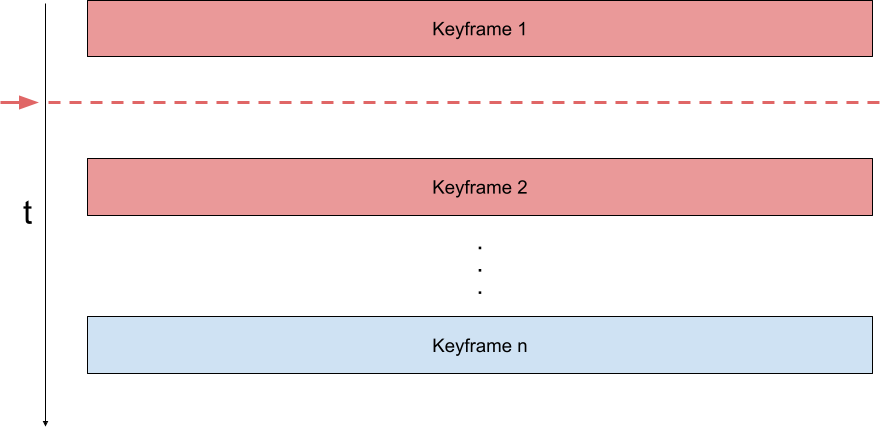
\includegraphics[width=0.6\linewidth]{../common/03_billiard_ai/resources/31_keyframe_animation.png}
    \end{center}
    \caption{Keyframe Animation}
    \label{fig:keyframe_animation}
\end{figure}

Das Animationsmodell wird anhand des Simulationsmodells abgeleitet. Dazu kann Abbildung
\ref{fig:simulationsmodell_keyframes} betrachtet werden. Wie in Kapitel \ref{kap:physikalisches_system} erklärt, besteht
das physikalische Simulationsmodell aus in Layern gruppierte Knoten. Diese Knoten haben jeweils eine Eingabe- wie auch
eine Ausgabeschicht. Eine Gruppierung dieser Knoten in einem Layer weist dadurch dieselbe Eigenschaft auf.

\begin{figure}[h!]
    \begin{center}
        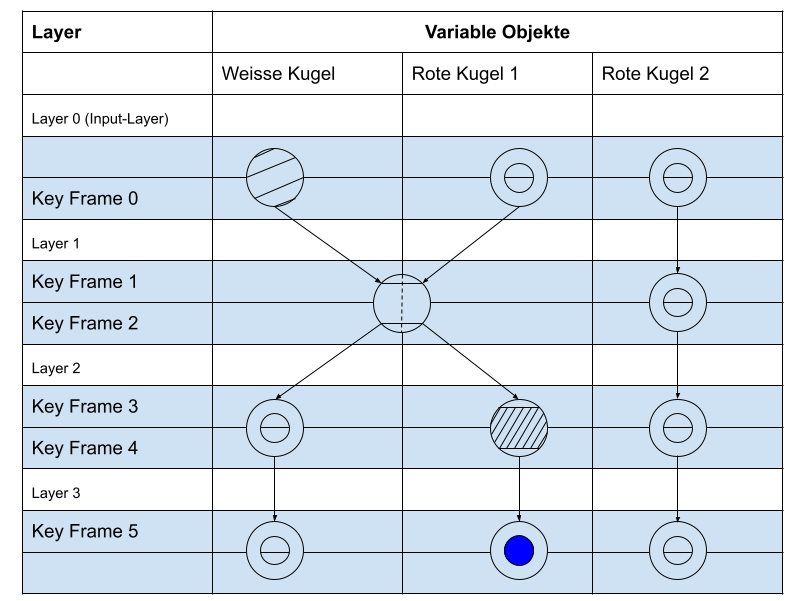
\includegraphics[width=0.6\linewidth]{../common/03_billiard_ai/resources/18_animation_keyframes.png}
    \end{center}
    \caption{Simulationsmodell mit Keyframes}
    \label{fig:simulationsmodell_keyframes}
\end{figure}

Jede Eingabe- wie auch Ausgabeschicht bildet so im Animationsmodell ein Keyframe. Die Besonderheit liegt darin, dass
nicht wie bei einer nach Lehrbuch aufgebauten Keyframe-Animation mit Fortlaufen der Zeit die Keyframes durchiteriert
\footnote{Durchiterieren bedeutet, dass wenn ein Keyframe vorher das Ende markierte, wie es das Keyframe 2 in Abbildung \ref{fig:keyframe_animation} tut, dann wird
das Keyframe 2 mit Fortlaufen der Zeit zum Startkeyframe und das nächstfolgende zum neuen Ende.} werden. Die Keyframes, welche aufgrund
des Simulationsmodells generiert werden, werden paarweise als Fenster betrachtet. Dieses Paarfenster wird bei Erreichen
des Endkeyframes auf das nächste Paar verschoben. Die Funktionsweise ist in Abbildung \ref{fig:simulationsmodell_keyframe_paare}
beschrieben. Dort werden die verschiedenen Keyframefensterpaare unterschiedlich rot markiert. Die Zeit schreitet wiederum in
vertikaler Richtung nach unten voran, der rote Pfeil auf der linken Seite zeigt eine mögliche aktuelle Position innerhalb
einer Animation. Demnach wäre das zweite Keyframefenster mit den Keyframes 2 und 3 aktiv.

\begin{figure}[h!]
    \begin{center}
        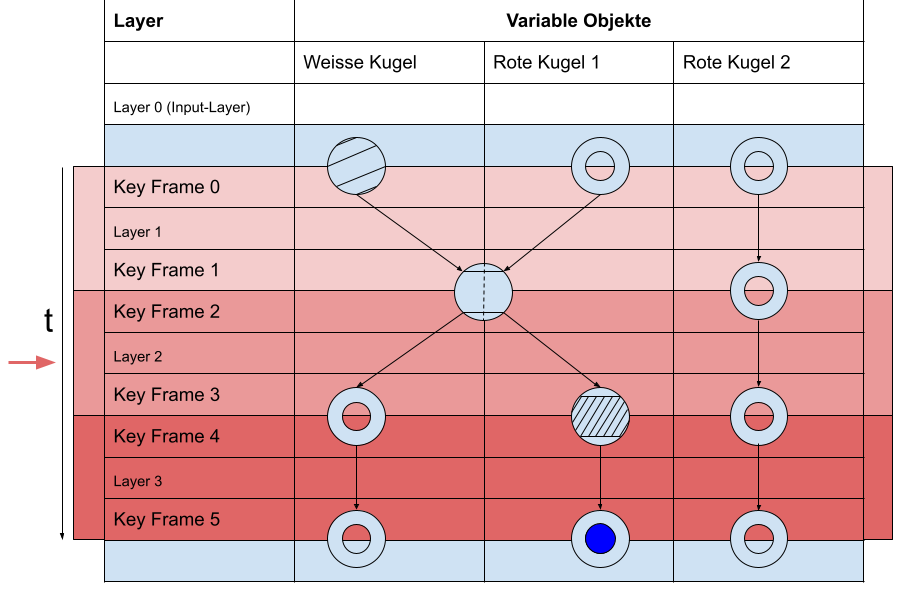
\includegraphics[width=0.6\linewidth]{../common/03_billiard_ai/resources/32_simulation_animationfenster.png}
    \end{center}
    \caption{Simulationsmodell mit paarweisen Keyframefenstern}
    \label{fig:simulationsmodell_keyframe_paare}
\end{figure}

Die Begründung der etwas spezielleren Handhabung liegt an der Tatsache, dass bei einem physikalischen Ereignis wie
einer Kugelkollision eine Veränderung des Status geschieht. So werden im Wesentlichen die Magnituden wie auch die
Richtungen der Geschwindigkeitsvektoren verändert. Würde nur ein Keyframe bei einem solchen Ereignis generiert werden,
dann könnte nicht mehr zwischen den Geschwindigkeitsvektoren aufgrund der geänderten Richtung interpoliert werden.

Die so generierte Animation kann als Gruppierung von einzelnen Keyframeanimationen, wie in Abbildung \ref{fig:keyframe_animation}
angegeben, mit jeweils nur zwei Keyframes angesehen werden.
\newpage
\subsection{Tiefensuche}
Um dem Spieler einen möglichst optimalen Stoss vorzuschlagen, sollte nicht nur der aktuelle Spielstand,
sondern auch die zukünftigen Spielstände und deren mögliche Stösse berücksichtigt werden.
Ein Stoss ist nur gut, wenn er für die Darauffolgenden eine ebenso gute, wenn nicht bessere, Ausgangslage bietet.
Ein guter Stoss in der aktuellen Situation kann evtl. zu schwierigeren Stössen führen, weil der Spielball schlecht platziert wurde.
Daher wurde beim Lösungsdesign des Suchalgorithmus darauf geachtet, dass eine Suche über mehrere Stösse ermöglicht wird.
Es handelt sich immer noch um eine Graphensuche, deren Suchraum jedoch erweitert wird.
Ein korrespondierender Suchbaum wird in Abbildung \ref{fig:suchbaum_tiefensuche} veranschaulicht.
Die orangenen Knoten bilden die Root-Knoten, die Repräsentation der Ziellöcher. Die grünen Knoten sind
Expansionsknoten. Diese stehen z.B. für einen Weg über eine Kugel oder eine Bande. Die beiden Knoten sind bereits aus
Kapitel \ref{sec:kandidatensuche} bekannt. Sobald die weisse Kugel expandiert wird, ist eine Kandidatensuche beendet und
es startet eine Simulation. Die Simulation wird beim Durchführen des Suchalgorithmus ebenfalls als Knoten in diesem
Suchbaum angesehen, hier blau eingefärbt. Nach der Berechnung eines Simulationsknotens kann die Suche bei genügender
Tiefe beendet oder wie in Ebene 3 fortgeführt werden. Das Resultat des Simulationsknotens bildet den neuen Spielstand
und es werden neue Root-Knoten darauf basierend expandiert. Die Suche kann so zukünftige Stösse in die Bewertung
des aktuellen Stosses einbeziehen.
Das Resultat der Tiefensuche sind nicht mehr nur einzelne Stösse, sondern Abfolgen von Stössen, welche nacheinander
ausgeführt werden könnten.

\begin{figure}[h!]
    \begin{center}
        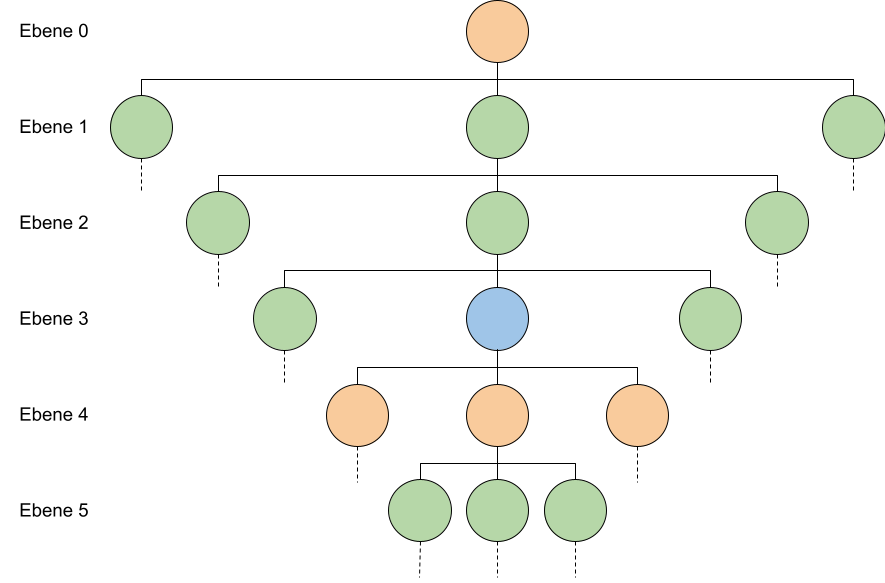
\includegraphics[width=0.5\linewidth]{../common/03_billiard_ai/resources/38_tiefensuche_suchbaum.png}
    \end{center}
    \caption{Suchbaum der Tiefensuche}
    \label{fig:suchbaum_tiefensuche}
\end{figure}

\subsubsection{Regeln für Snooker}\label{kap:tiefensuche:regeln_fuer_snooker}
Wird über mehrere Stösse gesucht, sind gewisse Regeln des Spiels einzuhalten. Bei Snooker werden abwechslungsweise rote
und farbige Kugeln versenkt, solange noch rote Kugeln auf dem Tisch sind. Die farbigen Kugeln haben unterschiedliche
Werte: Gelb(2), Grün(3), Braun(4), Blau(5), Pink(6), Schwarz(7)\cite{stoppball:spielregel:snooker}.\\
Gibt es noch eine oder mehrere rote Kugeln zu spielen, wird die versenkte farbige Kugel, ausser Rote, wieder
auf ihrem Spot (Aufsetzmarke) platziert. Ist der Spot nicht frei, so wird sie auf den nächst höherwertigen Spot gelegt. Die Wertung
der Spots entspricht der Wertung der Kugeln, welche bei der Ausgangsstellung platziert wurden. Die Ausgangsstellung ist in
Abbildung \ref{fig:snooker_ausgangslage} veranschaulicht. Wenn alle Spots belegt sind, wird die Kugel so nah wie möglich an ihrem ursprünglichen
Spot in Richtung der Kopfbande\footnote{Die Kopfbande ist diejenige, welcher der schwarzen Kugel bei der Ausgangstellung am
nächsten ist.} platziert\cite{stoppball:spielregel:snooker}.

\begin{figure}[h!]
    \begin{center}
        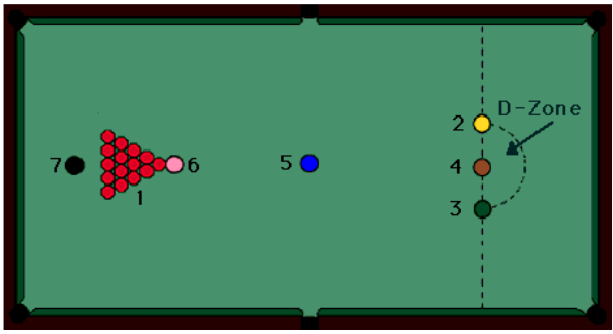
\includegraphics[width=0.4\linewidth]{../common/03_billiard_ai/resources/39_snooker_ausgangslage.png}
    \end{center}
    \caption{Ausgangslage bei Snooker\cite{stoppball:spielregel:snooker}}
    \label{fig:snooker_ausgangslage}
\end{figure}

Diese möglichst nahe Platzierung wurde über eine Suche nahe des Spots in einem diskretisierten Raum implementiert.
Abbildung \ref{fig:snooker_spot_replacement} veranschaulicht eine solche Situation, in der die Position $s$ besetzt
ist und daher eine möglichst nahe Platzierung erforderlich ist.
Es wird angenommen, dass sich die Kopfbande auf der rechten Seite befindet. Demnach wird zuerst eine Position in dieser
Richtung geprüft, danach eine Position in senkrechter Richtung zur Kopfbande und anschliessend die Position entgegengesetzt
zur Kopfbande.
Dies ist in Abbildung \ref{fig:snooker_spot_replacement} in den Schritten $1a$ bis $1d$ zu sehen.
Die Fringe $f$ beinhaltet potentielle Positionen für die zu platzierende Kugel, die noch auf Verfügbarkeit geprüft werden müssen.
Zu Beginn enthält $f$ nur die belegte Position $s$.
Ist eine Platzierung nicht möglich, werden die Positionen $a_1$ bis $a_4$ als neue Fringe betrachtet. Danach werden die Positionen
innerhalb der Fringe wiederum zuerst Richtung Kopfbande, danach in senkrechter Richtung zu dieser und anschliessend noch entgegengesetzt
auf Verfügbarkeit geprüft. Zu sehen in den Schritten $2a$ bis $2d$. Dies wird fortgeführt, solange die Kugel nicht platziert
werden konnte und die möglichen Positionen nicht zu weit vom Spot entfernt sind oder ausserhalb des Tisches liegen.
Wenn die Kugel nicht platziert werden konnte, wird dies als Fehler betrachtet und die Suche wird abgebrochen.

\begin{figure}[h!]
    \begin{center}
        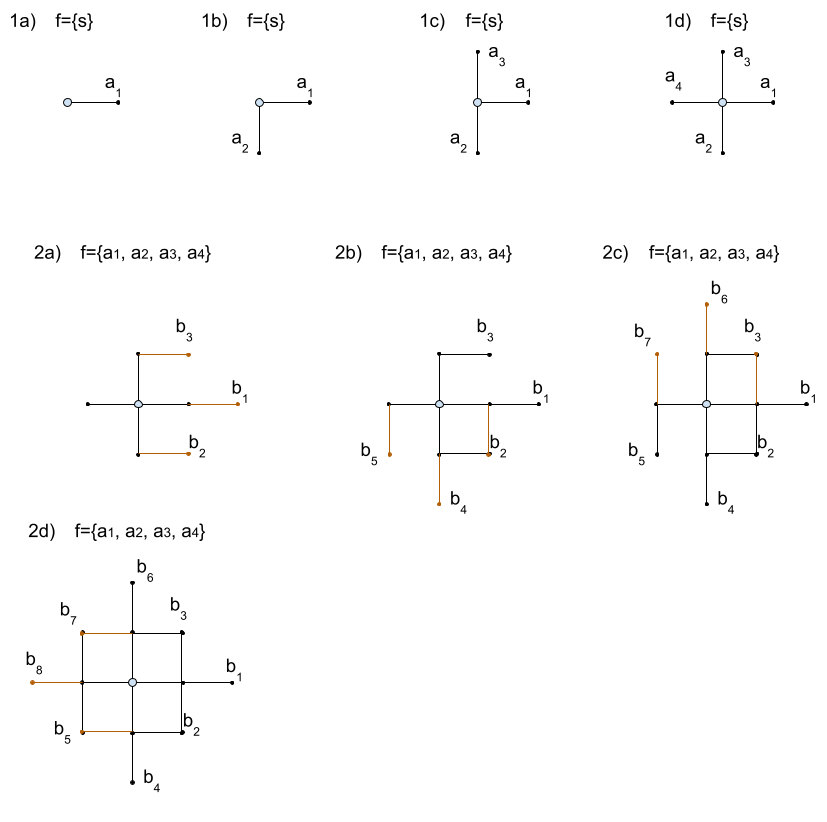
\includegraphics[width=0.6\linewidth]{../common/03_billiard_ai/resources/40_replatzierung_kugel.png}
    \end{center}
    \caption{Replatzierung einer Kugel nahe am Spot $s$}
    \label{fig:snooker_spot_replacement}
\end{figure}

Gibt es keine roten Kugeln mehr, werden die farbigen Kugeln in der Reihenfolge ihrer Punkte aufsteigend,
also Gelb, Grün, Braun, Blau, Pink, Schwarz versenkt und das Spiel ist beendet\cite{stoppball:spielregel:snooker}.

\newpage
\section{Berechnungsprozess}
Die Berechnung eines optimalen Stosses wird aufgrund der vielen Möglichkeiten sehr zeitintensiv, weswegen
die expandierten Teilschritte parallel gerechnet werden.

\begin{figure}[h!]
    \begin{center}
        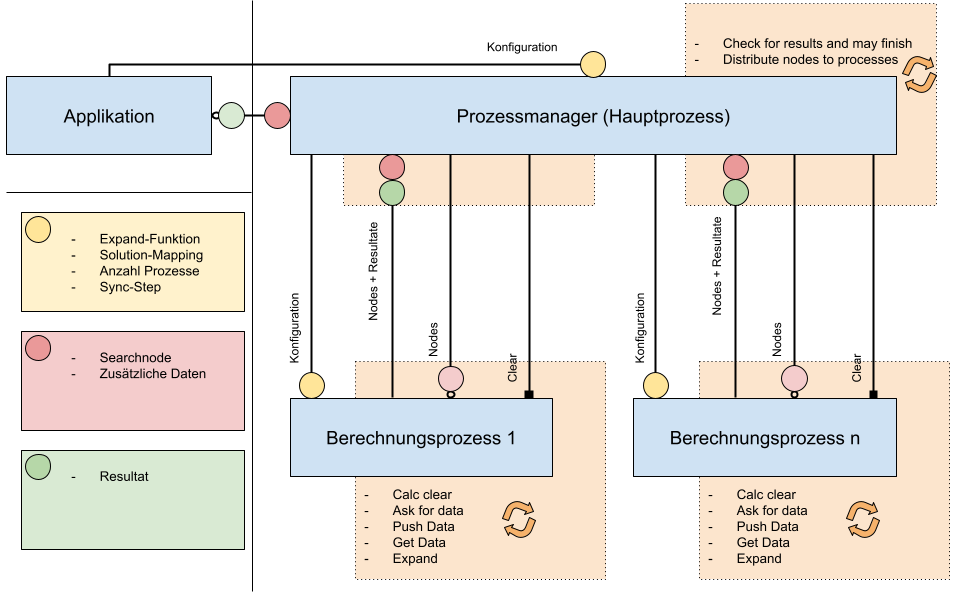
\includegraphics[width=0.8\linewidth]{../common/03_billiard_ai/resources/14_berechnungsprozess.png}
    \end{center}
    \caption{Berechnungsprozess}
    \label{fig:berechnungsprozess}
\end{figure}

Abbildung \ref{fig:berechnungsprozess} erläutert die Durchführung dieser Expansionsschritte.
Die Applikation auf der linken Seite liefert die konkreten Aufgaben, welche von einem Pool an Berechnungsprozessen
bearbeitet werden sollen. Sie beinhaltet die Logik, um eine solche Aufgabe zu lösen, da die Berechnungsprozesse
selbst nicht über dieses Wissen verfügen.
Der Pool von Berechnungsprozessen wird vom Prozessmanager verwaltet und dieser ist die zentrale Ansprechperson der Applikation.

Datenaustausche sind über gefärbte Kreise repräsentiert. Handelt es sich um einen asynchronen
Datenaustausch, dann ist der entsprechende Kreis heller eingefärbt und die Verbindungslinie ist durch einen nicht
ausgefüllten Punkt gekennzeichnet. Es werden die Farben Rot den zu bearbeitenden Daten,
Gelb den Konfigurationsdaten und Grün den Resultaten zugeordnet. Signale sind durch ein ausgefülltes Quadrat an der
Verbindungslinie gekennzeichnet. Das Signal oder die Daten sind jeweils beim Empfänger angegeben. Repetitive Aufgaben
sind durch ein hinterlegtes oranges Rechteck markiert.

Bei der Erstellung des Prozessmanagers werden alle Konfigurationen mitgeliefert. Der Prozessmanager erzeugt während seiner
Instanziierung die Prozesse, welche ebenfalls direkt konfiguriert werden. Die Prozesse laufen nun im Hintergrund und
warten auf Daten.

Erhält die Applikation eine Suchanfrage, ruft sie in einem ersten Schritt den Prozessmanager auf.
Dieser nimmt noch zu berechnende Daten entgegen. Im Fall von Billard sind dies die Root-Nodes des Suchbaums.
Jeder Root-Node repräsentiert ein Loch. Der Prozessmanager gibt in dem Fall eine Datenstruktur zurück, welche es erlaubt,
in Zukunft auf die Anfrage zu antworten. In dieser Antwort werden die Resultate geliefert.
Der Hauptprozess prüft regelmässig, ob die Bearbeitung der gestellten Aufgaben beendet werden soll.
Dies ist der Fall, wenn entweder genügend Lösungen gefunden wurden, die maximal zur Verfügung stehende Zeit abgelaufen ist
oder keine noch zu expandierenden Nodes mehr vorhanden sind.
Sollte die Berechnung nicht abgebrochen werden, dann werden die offenen Anfragen der Berechnungsprozesse beantwortet.
Der Prozessmanager verteilt alle ihm gemeldeten noch zu bearbeitenden Daten an die einzelnen Berechnungsprozesse.

In Abbildung \ref{fig:berechnungsprozess_verteilung} wird das Ziel verdeutlicht, welches der Prozessmanager bei einer
Verteilung dieser Daten verfolgt. So sollen die jeweils $n$ besten Kandidaten, wobei $n$ für die Anzahl der Berechnungsprozesse
steht, auf die verschiedenen Berechnungsprozesse verteilt werden. Danach erhalten die Berechnungsprozesse die nächstbesten
$n$-Kandidaten. Dadurch wird sichergestellt, dass immer an den vielversprechendsten Arbeitspaketen weitergemacht wird.

\begin{figure}[h!]
    \begin{center}
        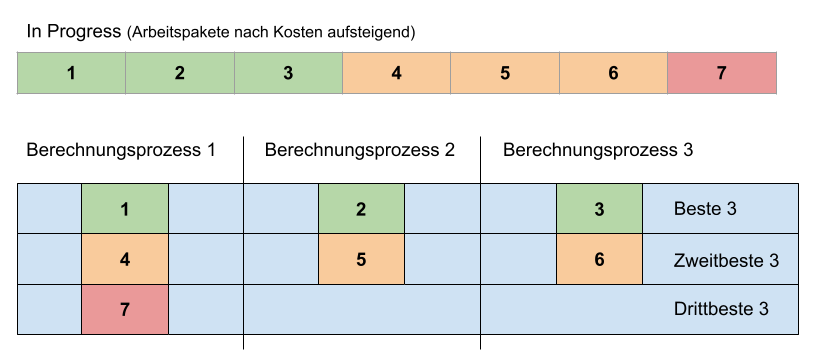
\includegraphics[width=0.8\linewidth]{../common/03_billiard_ai/resources/20_berechnungsprozess_verteilung.png}
    \end{center}
    \caption{Berechnungsprozessverteilung}
    \label{fig:berechnungsprozess_verteilung}
\end{figure}

Der Algorithmus \ref{alg:distribute_manager} zeigt, wie die offenen Arbeitspakete auf die Berechnungsprozesse verteilt
werden, damit das Ziel in Abbildung \ref{fig:berechnungsprozess_verteilung} erreicht werden kann. So werden
zuerst alle Antworten auf die offenen Anfragen erstellt. Dies geschieht in einer \glqq While-Loop\grqq, welche so lange
läuft, wie es noch offene Arbeitspakete hat. In jedem Schritt der Schleife wird ein Arbeitspaket einer Antwort für eine
Anfrage hinzugefügt. Am Ende der Schleife wird eine Index-Variable hochgezählt. Sollte diese die Anzahl der offenen Anfragen
erreichen, beginnt sie wieder bei 0. Dies ist z.B. in Abbildung \ref{fig:berechnungsprozess_verteilung} beim Wechsel von
Arbeitspakte $3$ zu $4$ ersichtlich. Sobald keine offenen Arbeitspakete mehr existieren, werden sämtliche Anfragen
beantwortet, zu welchen Antworten erstellt werden konnten. Wenn z.B. mehr Anfragen als Arbeitspakete existieren, bleiben
diese erhalten und werden im nächsten Synchronisationszyklus beantwortet\footnote{Man stelle sich bei der Abbildung
\ref{fig:berechnungsprozess_verteilung} nur zwei offene Arbeitspakete vor. Demnach würde Paket $1$ auf den Berechnungsprozess
    $1$ und Paket $2$ auf den Berechnungsprozess $2$ verteilt werden. Die Anfrage des Berechnungsprozesses $3$ bliebe offen.}.
\begin{algorithm}[H]
    \DontPrintSemicolon
    \SetKwFunction{distribute}{distribute}
    \SetKwProg{Fn}{Function}{}{}
    \Fn{\distribute{requests: List[future], inProgress: Queue[Node]} $\longrightarrow$ List[future]}{
        answers: List[List[Node]] $\longleftarrow$ list()\\
        forRequest $\longleftarrow$ 0\\
        \While{! inProgress.empty()}{
            \If{answers[forRequest] is null}{
                answers[forRequest] = list()
            }

            node $\longleftarrow$ pop(inProgress)\\
            answers[forRequest] $\longleftarrow$ append(node, answers[forRequest])\\
            forRequest $\longleftarrow$ (forRequest + 1) \% size(requests)
        }

        \While{! answers.empty()}{
            request $\longleftarrow$ pop(requests)\\
            fulfill(request, pop(answers))
        }

        \KwRet requests
    }
    \caption{Algorithmus zur Durchführung eines Expansionsschritts im Berechnungsprozess}
    \label{alg:distribute_manager}
\end{algorithm}

In einem Zyklus eines Berechnungsprozesses wird zuerst geprüft, ob eine Berechnung abgebrochen werden soll. Dies ist der
Fall, wenn der Prozessmanager ein \glqq Clear-Signal\grqq{} gesendet hat. Dieses Signal tritt auf, wenn eine neue
Berechnung gestartet oder wenn eine aktuell Laufende erfolgreich beendet oder abgebrochen wird.

Der Berechnungsprozess stellt in einem nächsten Schritt eine Datenanfrage an den Prozessmanager, sollte keine offene oder
noch nicht bearbeitete Anfrage existieren. Danach erfolgt die Prüfung, ob die Zeit zwischen einem Synchronisationsschritt
abgelaufen ist. In dem Fall liefert der Berechnungsprozess seine besten weiterzuführenden Berechnungen wie auch Resultate
dem Prozessmanager. Er wird demnach für eine Weile an weniger erfolgversprechenden Resultaten weiterarbeiten. In einem
weiteren Schritt wird geprüft, ob eine Datenanfrage bereits beantwortet wurde. Ist dies der Fall, so werden die
Daten den zu bearbeitenden Daten des Berechnungsprozesses hinzugefügt. Zuletzt erfolgt der Expansionsschritt, wobei der
erfolgversprechendste Kandidat expandiert wird.
Der Algorithmus \ref{alg:expand_berechnung} zeigt, wie dies in etwa funktionieren kann.
Als Eingabe dient eine priorisierte Queue von offenen Arbeitspaketen sowie die Implementation der \glqq Expand-Funktion\grqq.
Wenn es offene Arbeitspakete gibt, dann wird das Beste genommen und über die Implementation der
\glqq Expand-Funktion\grqq{} expandiert. Das Resultat dieses Schrittes wird danach entweder den Lösungen oder den
offenen Arbeitspaketen hinzugefügt. Am Schluss werden die offenen Arbeitspakete wie auch die Lösungen zurückgegeben.

\begin{algorithm}[H]
    \DontPrintSemicolon
    \SetKwFunction{expand}{expand}
    \SetKwProg{Fn}{Function}{}{}
    \Fn{\expand{inProgress: Queue[Node], expandImpl: functional} $\longrightarrow$ Queue[Node], Queue[Node]}{
        solutions $\longleftarrow$ priority\_queue()\\
        \If{!inProgress.empty()}{

            node $\longleftarrow$ pop(inProgress)\\
            expandedNodes $\longleftarrow$ expandImpl(node)\\

            \For{expandedNode in expandedNodes}{
                \If{expandedNode.isSolution()}{
                    solutions $\longleftarrow$ append(expandedNode, solutions)
                }
                \Else{
                    inProgress $\longleftarrow$ append(expandedNode, inProgress)
                }
            }
        }

        \KwRet inProgress, solutions
    }
    \caption{Algorithmus zur Durchführung eines Expansionsschritts im Berechnungsprozess}
    \label{alg:expand_berechnung}
\end{algorithm}

Die Synchronisation zwischen den Prozessen wird in Abbildung \ref{fig:berechnungsprozess_synchronisation} erläutert.
Sie findet nach einer konfigurierten Zeit $k$ statt. Diese wird in Millisekunden $[ms]$
angegeben. Da die Synchronisation ein exklusives Verwenden einer geteilten Ressource erfordert, um die erledigte Arbeit
dem Prozessmanager mitzuteilen, erhalten alle laufenden Prozesse (dies umfasst den Hauptprozess des Prozessmanagers wie auch
alle Berechnungsprozesse) ein Zeitfenster zugeteilt, welches nach $k$ Millisekunden startet. Danach kann jeder Prozess nach
$k + i \cdot n$, wobei $i$ für die Prozess-ID beginnend bei $0$ und $n$ für das Zeitfenster einer Synchronisation steht,
mit der Synchronisation beginnen. Es wird so verhindert, dass zu viele Prozesse auf die Ressource des Prozessmanagers
warten müssen und untätig bleiben. Ein weiterer Vorteil dabei ist die Tatsache, dass in der Zeit der Synchronisation
einige Prozesse Zeit erhalten, um eher schlechter bewertete Kandidaten weiterzuverfolgen. Dadurch ist es möglich,
dass ein sehr gutes Ergebnis gefunden werden kann, obwohl dessen Kandidat anfänglich als schlecht beurteilt wurde.

\begin{figure}[h!]
    \begin{center}
        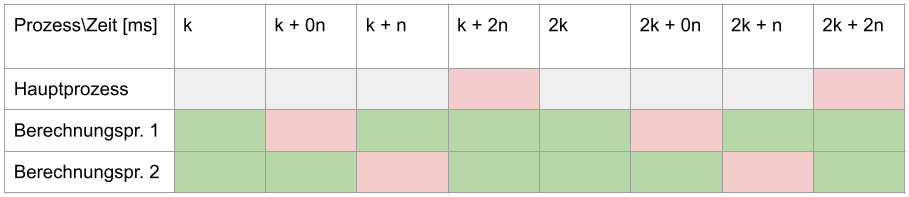
\includegraphics[width=0.8\linewidth]{../common/03_billiard_ai/resources/15_berechnungsprozess_synchronisation.png}
    \end{center}
    \caption{Berechnungsprozesssynchronisation}
    \label{fig:berechnungsprozess_synchronisation}
\end{figure}

Die Abbildung \ref{fig:berechnungsprozess_synchronisation} zeigt den Hauptprozess wie auch zwei Berechnungsprozesse, welche
eine Synchronisation in einem Intervall von $k$ Millisekunden durchführen. Grüne Spalten stehen hierbei für die Zeit, welche für die Berechnung
einer Lösung verwendet wird, also als produktiv bezeichnet werden kann. Rote Spalten hingegen signalisieren den unproduktiven
Overhead, der bei der Synchronisation entsteht. Der Prozessmanager macht nebst seinem Synchronisationsfenster nichts,
weswegen seine Spalten grau markiert sind. Eine mögliche Verbesserung wäre die Auslastung des Prozessmanagers mit zusätzlicher
Berechnungsarbeit, wie sie die Berechnungsprozesse durchführen.
